\documentclass[12pt]{article}
\usepackage{amsmath}
\usepackage{amsfonts}
\usepackage{amssymb}
\usepackage{graphics}
\usepackage{graphicx}
\usepackage{wrapfig}
\usepackage{titlesec}
\usepackage{xcolor}
\usepackage{enumitem}
\usepackage[bottom]{footmisc}
\usepackage{tabularx}
\usepackage{float}
\usepackage{multirow}
%\newcommand{\sectionbreak}{\clearpage}
%\usepackage[margin=0.5in]{geometry}

\usepackage{fancyhdr}
\usepackage[left=1.5cm, right=1.5cm, top=2cm, bottom=1.5cm]{geometry}

\pagestyle{fancy}
\fancyhf{}
\rhead{}
\lhead{\small{\rightmark}}
\lfoot{\textcolor{gray}{\small{Aurelio Marin, Edoardo Peretti, Luca Pirazzini}}}
\rfoot{\thepage}

\setlength{\headheight}{13.6pt}


\begin{document}
	\title{%
		Analysis of Spatially Correlated Bike Sharing Demand in New York City \\ \vspace{3 mm}}
		%\large Use of bike sharing in New York City}
	\author{Aurelio Marin, Edoardo Peretti, Luca Pirazzini}
	\date{February 19, 2020}
	
	\maketitle
\vspace{10 mm}

\begin{abstract}
	The most general purpose of this work is to model patterns between observed data distributed over a spatial environment that are characterized by autocorrelation. Usually such data consist in measurements of some quantity of interest, which in plenty of practical cases is likely to be a demand of a good. 
	In the conduction of this, following an exploratory analysis of autocorrelation we introduce a general geostatistical linear regression model, following a Bayesian approach, describing its components and the assumptions needed in order to apply it to the context of data on bike sharing demand in New York City, and assessing how such demand is affected by other external factors. 
	By evaluating the effects of a few different spatially referenced regressors over two different training sets, we proceed with a qualitative comparison between models, also using some common predictive goodness of fit criteria in Bayesian analysis. Finally, as a model validation tool, predictive performance of such models on a different subset of data is discussed.
\end{abstract}	

\newpage
\tableofcontents

\newpage
\section{Introduction: New York City Bike Sharing}
\noindent
CitiBike \cite{stationdata} is the largest bike sharing system of New York City, NY as far of fleet size and coverage extension. By considering its operations as point-to-point, it serves the almost entire Manhattan area, plus a part of Brooklyn and Queens. Manhattan accounts for the largest population in the country and one of the absolute largest in the world during daytime, with 4 million individuals among commuting workers, students, residents, and visitors. This should be an important motivation to consider a bicycle as an efficient way to cover small to medium every-day commutes, given the dense environment of the city. Currently CitiBike includes more than 700 stations. In our work, we have restricted the focus on Manhattan, as data were easier to retrieve and the area covered seems to be large enough to capture interesting effects.\\

\noindent
The main variable of interest, in the course of the analysis, will be the number of trips departing a specific station, or simply demand from a station. The data used on this are relative to the month of November, 2017.
Figure \ref{manhattan_demand} shows the distribution of the demand in Manhattan.


\begin{figure}[H]
	\centering
	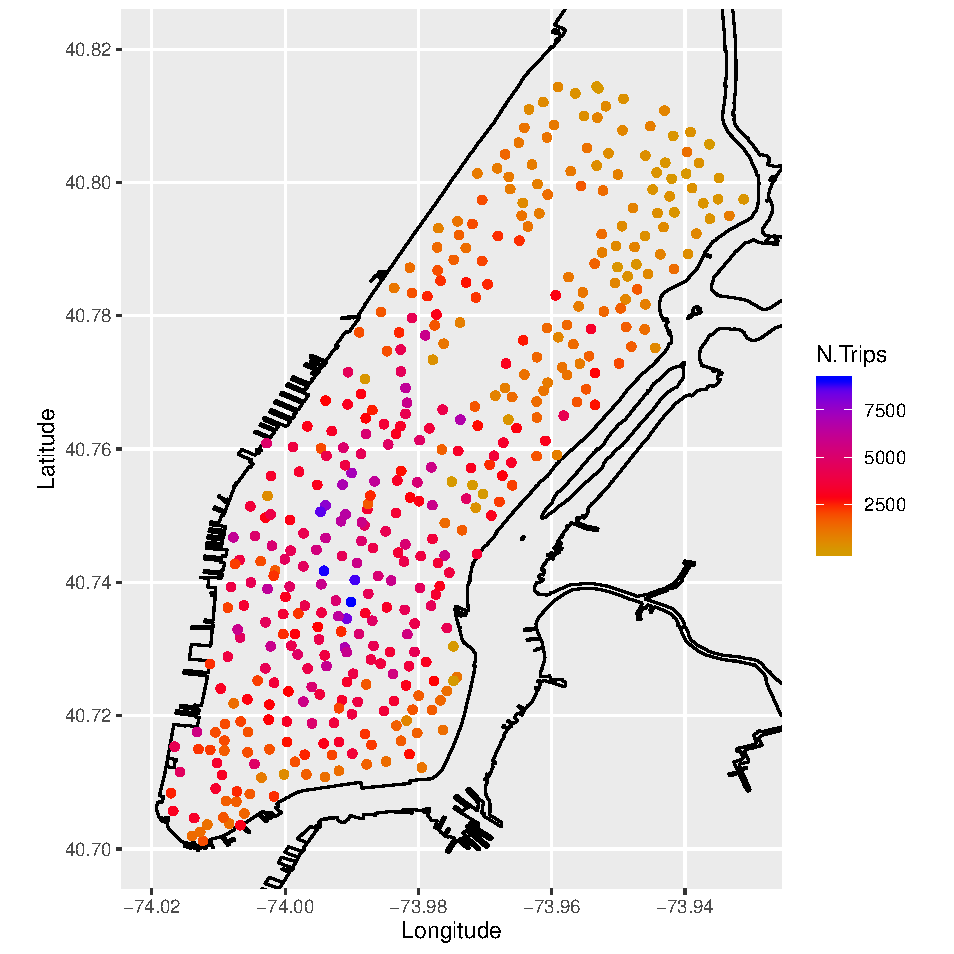
\includegraphics[scale=.9]{Pictures/solomanhattan.pdf}\\
	\caption{Map of CitiBike stations in Manhattan, colored according to monthly number of trips} \label{manhattan_demand}
\end{figure}


\section{Preliminary analysis of Spatial Autocorrelation}

One of the key points of working with spatially distributed data is autocorrelation. In complex problems, spatial autocorrelation is multi-directional and multi-dimensional. It can also be very sensitive to the amount of data actually considered, and to the size of the spatial domain.
The most common way to assess any kind of significant association between data observed at different locations is to compute proper indicators. Here we briefly present two of them: Moran's I and Geary's C.
	
\subsection{Moran's Index I}
The Moran's I index is defined as 
$$
	I = \displaystyle{\frac{N\displaystyle\sum_{i=1}^{N} \sum_{j=1}^{N} W_{ij}(x_{i}-\overline{x})(x_{j}-\overline{x})}{\displaystyle\sum_{i=1}^{N}\sum_{j=1}^{N} W_{ij}\displaystyle\sum_{i=1}^{N} (x_{i}-\overline{x})^2}}
$$
$N$ number of observations\\
$\overline{x}$ sample mean of all the observations\\
$W_{ij}=\textstyle\frac{1}{d_{ij}}$ weight matrix, with $d_{ij}$ distance between points $i,j$ \\

\noindent
Moran's I is mostly suitable for checking global autocorrelation of a set of data. The index evaluation is subject to a significance test where $H_0 : $ no spatial autocorrelation. Namely, under $H_0$ data values are randomly distributed, according to no pattern.\\

\noindent
The null hypothesis equivalently sets an expected, or default, value for I equal to $\textstyle-\frac{1}{(N-1)}$.
As such default value merely depends on the number of observations, this is just a remark of the fact that a larger N means, by chance, a higher probability of randomness and absence of patterns between observed values. Therefore, an expected I close to 0 means no autocorrelation.
To actually evaluate autocorrelation, the computed I must be put into comparison with the expected I.

\begin{figure}[H]
\centering
\fbox{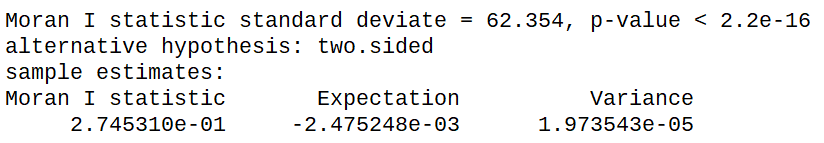
\includegraphics[scale=0.8]{Pictures/Moran_full.png}}\\
\end{figure}
\noindent
In testing this hypothesis on our dataset, the p-value is very low and the z-score (here as standard deviate) is large and positive. These facts show significant evidence to reject $H_0$, meaning presence of global spatial autocorrelation. 
Moreover, a positive value, far enough from 0, means that similar values tend to cluster together over a spatial domain. This fact agrees with the dynamics of the demand across the map. At least in most subcases, nearby stations will present close values.\\

\noindent
However, a ``perfect clustering" scenario would be achieved when Moran's I equals 1, therefore some exceptions cannot be neglected, and they are likely due to the presence of sites of major importance, according to the type of user.

\subsection{Geary's Index C}
The Gearys C index is defined as
$$
C = \displaystyle{\frac{(N-1)\displaystyle\sum_{i=1}^{N}\sum_{j=1}^{N} W_{ij}(x_{i}-x_{j})^{2}}{2\displaystyle\sum_{i=1}^{N}\sum_{j=1}^{N}W_{ij}\displaystyle\sum_{i=1}^{N}(x_{i}-\overline{x})^2}}
$$

\noindent
Geary's C instead, thanks to its numerator being a slightly different form, is more sensitive to the absolute difference between neighboring observations $x_i$ and $x_j$. Therefore it somewhat accounts also for the local autocorrelation structure.

	\begin{figure}[H]
	\centering
	\fbox{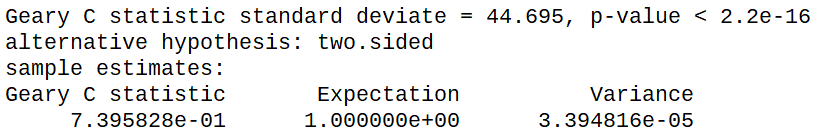
\includegraphics[scale=0.8]{Pictures/Geary_full.png}}
	\end{figure}

\noindent	
The results agree with those from Moran's I test. By construction 1 is the expected value of C, and a value between 0 and 1 for C means that observed demand at stations are clustered, rather than dispersed.
This seems to make sense. If a new station is added to the network within a close range of distance from an existing one, it is likely to catch an amount of demand that will be reasonably similar to that of the nearby station, eventually by ``stealing" some demand from it, but still reaching a reasonably close value afterwards.
	
\subsection{Moran autocorrelation plot}
In the Figure \ref{moran_plot}, a scatter plot of observed bike demand in Manhattan against its own spatially lagged values is shown. Points follow a positive autocorrelation pattern.
	
	\begin{figure}[H]
		\centering
		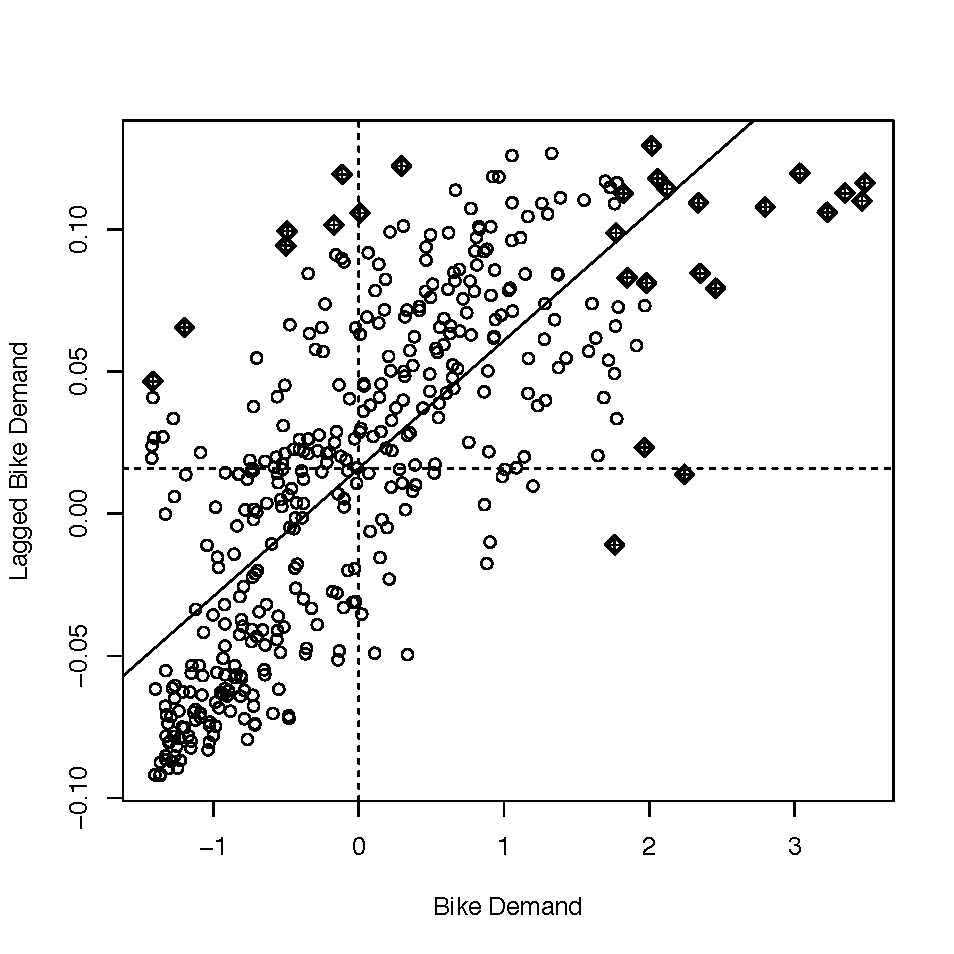
\includegraphics[scale=0.6]{Pictures/Moran_manhattan.pdf}
		\caption{Moran autocorrelation plot}\label{moran_plot}
	\end{figure}

\noindent
Autocorrelation is proven to be significant from the two tests, particularly when the number of observation considered becomes larger. Nonetheless, when performing a test on a strictly local scale (including very few stations such as 10 to 20), there are several cases in which Moran's I statistic value would suggest negative autocorrelation, i.e similar values are dispersed. In these cases, the p-value of the test is large, and the standard deviate quite small, which should mean that there is no longer evidence of a strong pattern between observations, and in a minor number of cases this happens by chance .
	
	
	%\begin{center}
		%\centerline{%
		%	\includegraphics[scale=0.5,width=0.5\textwidth]{Pictures/Moran_54stations2017.pdf}%
		%	\includegraphics[scale=0.5,width=0.5\textwidth]{Pictures/Moran_negcorr.pdf}%
		%}%
		%\begin{small}
		%	Examples of data subsets showing positive (left) and negative (right) autocorrelation, according to Moran's I
		%\end{small}
	%\end{center}
	

%Assuming observed demands as iid, the null hypothesis of the related test is \\
%$I \sim \mathcal{N}(-\frac{1}{N-1},Var(I))$ \\
%\vspace{2 mm}\\
%which means that there is evidence of spatial autocorrelation of demand when the I value is close to
%$-\frac{1}{N-1}$


\section{Point-referenced modeling approach}


The original structure of these data is point-referenced: the number of bikes at each station is associated to its own pair of coordinates (longitude and latitude). Thus the natural model that best suits such type of data is a Gaussian linear model.
	
	\subsection{Gaussian linear regression model}


Given a spatial domain $\mathcal{D} \subset \mathbb{R}^2$ and a finite set of points $\{\boldsymbol{s}_i : i = 1, \dots , n \}$, the observed demand $Y$ at location $\boldsymbol{s}_i$ is described as
$$\begin{large}Y(\boldsymbol{s}_i) = \mathbf{x}^\intercal (\boldsymbol{s}_i) \boldsymbol{\beta} + w(\boldsymbol{s}_i) + \varepsilon(\boldsymbol{s}_i) \end{large}$$ %\hspace{10 mm} $i = 1,\dots,n$\\
	%\vspace{1 mm}
	%$Y(\mathbf{s_i}) = \mathbf{x}^\intercal (\mathbf{s_i}) \boldsymbol{\beta} + w(\mathbf{s_i}) + \varepsilon(\mathbf{s_i})$, \hspace{10 mm}$i = 1,\dots,n$\\

\noindent
$\mathbf{x}^\intercal (\boldsymbol{s}_i)$ vector of spatially referenced predictors\\
$w(\boldsymbol{s}_i)$ stationary spatial process\\
$\varepsilon(\boldsymbol{s}_i)$ pure error term \\
	
\noindent
In order to adapt the common structure of a linear model to the context of geostatistical analysis, this model provided by the R function \emph{spLM} (package \emph{spBayes}) adds to the well known family of the regression parameters $\boldsymbol{\beta}$ and to the independent and identically normally distributed residual error terms $\varepsilon$ an underlying Gaussian spatial process $w$, that accounts for the variability of the full process due to interactions between observations over the spatial domain.
	

	\subsection{Discussing the model assumptions}

Before explaining in detail the full Bayesian description the model, there are two main properties that the spatial process $w$ is supposed to fulfill: intrinsic stationarity and isotropy.
	
	\subsubsection{Intrinsic stationarity}
	A spatial process \{$w(\boldsymbol{s}), \boldsymbol{s} \in \mathcal{D}$\} is intrinsic stationary if
	\begin{enumerate}[label=(\arabic*)]
		\item $\mathbb{E}[w(\boldsymbol{s}_i)]=C$ \hspace{5 mm} for any $\boldsymbol{s}_i \in \mathcal{D}$
		\item Var$[w(\boldsymbol{s}_i)-w(\boldsymbol{s}_j)] = 2\gamma(\mathbf{h})$ \hspace{5 mm} for any $\boldsymbol{s}_i$, $\boldsymbol{s}_j \in \mathcal{D}$, $\boldsymbol{h}= \boldsymbol{s}_i-\boldsymbol{s}_j$
	\end{enumerate}
	Property (1) states that the mean of the process shall be constant over the domain $\mathcal{D}$ considered, while (2) states that the variance of the difference between two observations of the process is a function of the only separation vector between the corresponding points, where $\gamma(\boldsymbol{h})$ denotes the semivariogram of the process.\\

\noindent
	Intrinsic stationarity, despite being the weakest form of stationarity, in most practical cases cannot be achieved by the response $Y(\boldsymbol{s}_i)$ over $\mathcal{D}$. It is clear that its mean will very rarely be constant over latitude and longitude. In \emph{spLM} the implementation $w$ provides partial adjustment (or smoothing) with a structured dependence to the mean at a local level.
	%From a very basic analysis in which the mean demand of bikes is computed with respect to latitude and longitude, it is possible to see that, overall, the mean is not close to be constant. \\
	%Its variability is lower in some selected areas, where the process might be seen as %intrinsic stationary since, as previously remarked, similar values may stick together, %thus the mean is less subject to big changes.
	
	
	
	\subsubsection{Isotropy}
	A spatial process \{$w(\boldsymbol{s}), \boldsymbol{s} \in \mathcal{D}$\} is isotropic if  Var$[w(\boldsymbol{s}_i)-w(\boldsymbol{s}_j)] = 2\gamma(d)$ \hspace{5 mm} for any $\boldsymbol{s}_i$, $\boldsymbol{s}_j \in \mathcal{D}$, $d =\left\lVert \mathbf{h} \right\rVert=\left\lVert \boldsymbol{s}_i-\boldsymbol{s}_j \right\rVert $. It is an equivalent, but stronger result than (2) since the variance of the difference between observations only depends on their absolute distance (modulus of the separation vector), regardless of the locations.\\

\noindent
	Isotropy in a two-dimensional framework can be checked using a nonparametric test from Maity and Sherman \cite{maity}. We checked if this property could be satisfied also by the response $Y$ of the model. This test is based on the comparison of sample covariogram with its estimation for specifics lags developing a test statistic based on the estimation of the asymptotic variance matrix.\\

\noindent
	The isotropy condition is represented by the null hypothesis  $H_0:\mathbf{A}\gamma(\Lambda)=\mathbf{0}$ where $\Lambda$ contains the specific lags for which the test is going to be carried and $\mathbf{A}$ is the contrast matrix that states how to make the comparison.\\

\noindent
	By choosing differents lags for various absolute distances and comparing orthogonal directions so as to get more variability, we have achieved a p-value of 0.85, meaning isotropy condition is met by $Y$ over areas within an approximate range of 1.5 km.
	This result could be corroborated by the representation of the semivariogram over different directions where we can appreciate that there is a similar behaviour for distance smaller than 1.5 km (Figure \ref{isotropy_plot}).
	
	\begin{figure}[H]
		\centering
		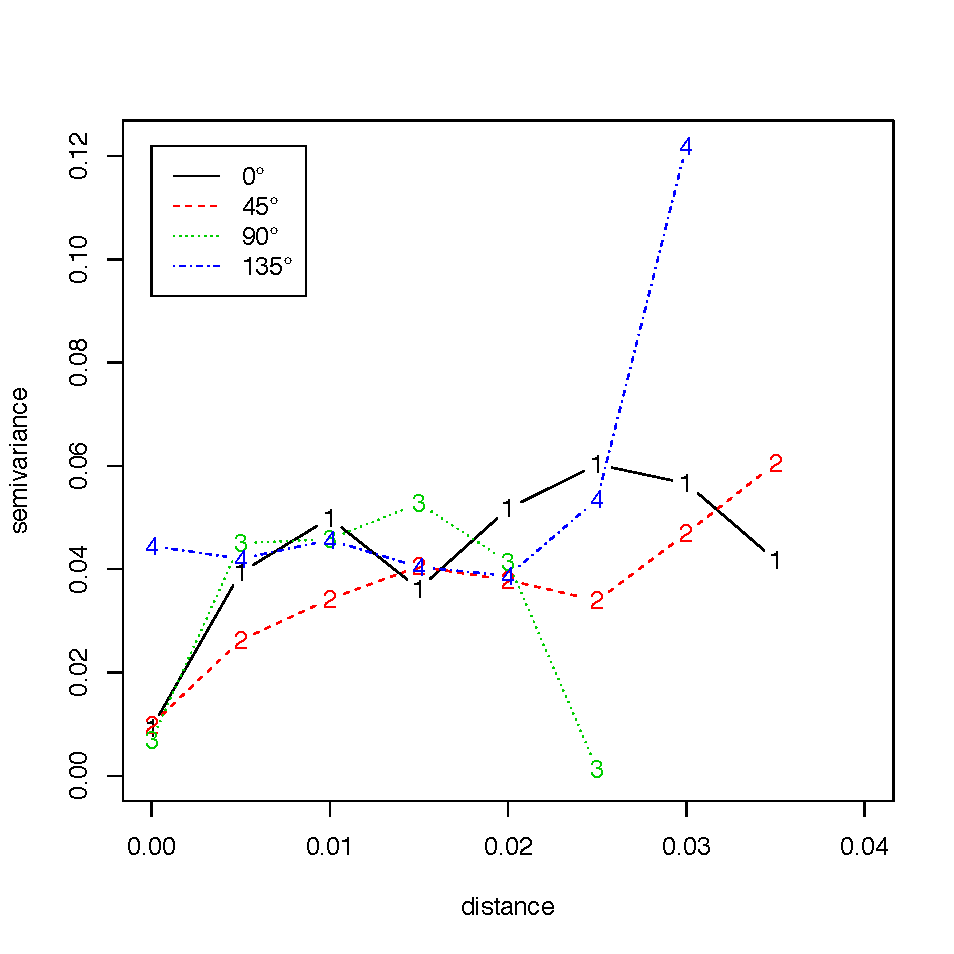
\includegraphics[scale=0.7]{Pictures/variogram_angle.pdf}\\
		\caption{Sample directional semivariograms}\label{isotropy_plot}
	\end{figure}

	\subsection{Bayesian hierarchical structure of the model}
	Denote the general covariance structure of the process with $C$. Under the assumption of isotropy consider $d=\left\lVert \mathbf{h} \right\rVert$. We first specify:
	\begin{itemize}
		\setlength\itemsep{2 mm}
		\item A set/vector of parameters $\boldsymbol{\theta} = (\boldsymbol{\beta}, \sigma^2, \phi, \tau^2)$
		\item An exponential covariance function
		$C(d;\sigma^2,\phi,\tau^2) = 
		\begin{cases}
		\text{$\sigma^2 e^{-\phi d}$} &\quad\text{$d > 0$}\\
		\text{$\tau^2+\sigma^2$} &\quad\text{$d = 0$}\\
		\end{cases}$
		\item Pure microscale errors $\varepsilon(\boldsymbol{s}_i)=\varepsilon_i \stackrel{i.i.d.}{\sim} \mathcal{N} (0,\tau^{2} ) $
	\end{itemize}
	The Gaussian linear model structure is
	\begin{align*}
	& Y|\mathbf{w},\boldsymbol{\beta},\tau^2 \sim \mathcal{N}(\mathbf{X}\boldsymbol{\beta} + \mathbf{w}, \tau^2 I) \\
	& \mathbf{w}|\sigma^2,\phi,\tau^2 \sim \mathcal{N}(\mathbf{0}, C(d;\sigma^2,\phi,\tau^2)) \\
	& \boldsymbol{\beta} \sim \mathcal{N}(\boldsymbol{\mu_\beta},\Sigma_\beta) \\
	& \sigma^2 \sim IG(a_1,b_1) \\
	& \tau^2 \sim IG(a_2,b_2) \\
	& \phi \sim \mathcal{U}(a_3,b_3) \\ %meglio non usare d perché indica anche la distanza (magari ppossiamo usare h (non in grassetto) per la distanza)
	& \pi(\boldsymbol{\theta}) = \pi(\boldsymbol{\beta})\pi(\sigma^2)\pi(\phi)\pi(\tau^2)
	\end{align*}
	
\noindent
More into the details, $\sigma^2$ is a spatial variance component of the Gaussian spatial process $w$, while $\phi$ is clearly a rate of correlation decay, in this case exponential. These two parameters represent the variability due to spatial structured dependence in the process.
	On the other hand $\tau^2$ is the variance of the random, non-spatial process, thus it describes the impact of external, non controllable effects of a model that always have to be considered in nature.
	
	\subsection{Prior hyperparameters choice and setup}
	The prior for the regression parameters $\pi(\boldsymbol{\beta})$ can be either flat (e.g Jeffrey's) or normally distributed. The posterior of $\boldsymbol{\beta}$ provided by the model using the \emph{spLM} function in R is expected to be normally distributed in both cases.\\

\noindent
	For both spatial and non-spatial associated variances $\sigma^2$ and $\tau^2$ the prior is typically distributed as an Inverse Gamma. Commonly the shape hyperparameters are set as $a_1 = a_2 = 2$ so that the mean of the distribution equals the scale hyperparameters, while the variance is infinite. The scale hyperparameters are chosen as: 
	\begin{itemize}
		\item $b_1$ proportion of residual variance from the spatial process $w$
		\item $b_2$ proportion of residual variance from the non-spatial process $\varepsilon$
	\end{itemize}
	The estimate of residual variance is obtained from the squared standard error of frequentist simple linear model fitting. In the models' performance we chose such proportions to be 80\% from the spatial process and 20\% from the non-spatial, giving a reasonably higher weight to the more interesting spatial effects.
The prior for the spatial decay parameter $\phi$ is instead given a Uniform distribution. 
The hyperparameters $a_3$ and $b_3$ are chosen according to
	\begin{itemize}
		\item $a_3 = -\displaystyle\frac{log(0.05)}{max\_dist}$ 
		\item $b_3 = -\displaystyle\frac{log(0.05)}{min\_dist}$
	\end{itemize}
	where $max\_dist$ and $min\_dist$ are the largest and smallest existing distance in the dataset considered in the model, that define an effective spatial range for the process. The value of 0.05 is suggested by Finley et al. \cite{spbayes} as a threshold value for correlation within the effective range.

	\section{Models for bike sharing data}

	
	\subsection{Choice of the predictors}
	For the point-referenced model we first selected a total of five predictors. In order to choose them, we based the computation and consequent assignment to each station in the dataset on the main fact that each station is uniquely distinguished from the others through its own latitude and longitude. Here there is list of their ``keyword", followed by a brief description:	
	\begin{itemize}
		\item \textbf{Population} : value provided for population according to 2010 Census to the block where a station is located \cite{populationdata}
		\item \textbf{Bike lanes} : number of bike lanes segments (as a quantitative measure) located within a range of 500 m from a station \cite{lanesdata}
		\item \textbf{Subway} : distance to the closest subway access from a station \cite{subwaydata}
		\item \textbf{Landmarks} : for each station, distance to the closest landmark\footnotemark
		\item \textbf{Proximity} : a score assigned to each station based on the sum of 	
		the square inverse distances from the other stations
	\end{itemize}
	Called $d_{ij}$ the distance (in meters) between $\boldsymbol{s}_i$ and $\boldsymbol{s}_j$ the proximity score is computed as
	$$Prox(\boldsymbol{s}_i) = \displaystyle\sum_{j:  \boldsymbol{s}_j \in \mathcal{D}}^{} \displaystyle\frac{1000}{{d_{ij}}^2}$$
	Population, lanes and subway predictors can be considered as major, global factors having an impact on a bike sharing usage. Subway, for instance, is the only transportation that competes with bike in terms of efficiency, in particular for short to medium trips over Manhattan, especially where bike lanes are easy to access.\\

\noindent
	Instead, we decided to compare separately the effects added by landmarks and proximity covariates, by fitting also models with just one of them, and with both.
	Indeed, the landmarks predictor focus is on tourists, while the proximity accounts for properties of centrality and closeness among stations. They were both added later with the aim of strenghtening the performance of the model.
	
	\footnotetext{Manhattan Landmarks: Central Park, Times Square, Empire State Building, Rockfeller Center, Brooklyn Bridge, High Line, Metropolitan Museum, OneWorld Trade Center}
	
	


\subsubsection{Correlation between predictors}

During the regression analysis, the employed predictors should be reasonably independent in order to avoid collinearity between them.
To check this property, we computed a correlation matrix for all the considered predictors.
As shown in Figure \ref{corrplot}, all the variables are weakly correlated to each other (all the correlations are below $0.4$).


\begin{figure}[H]
	\centering
	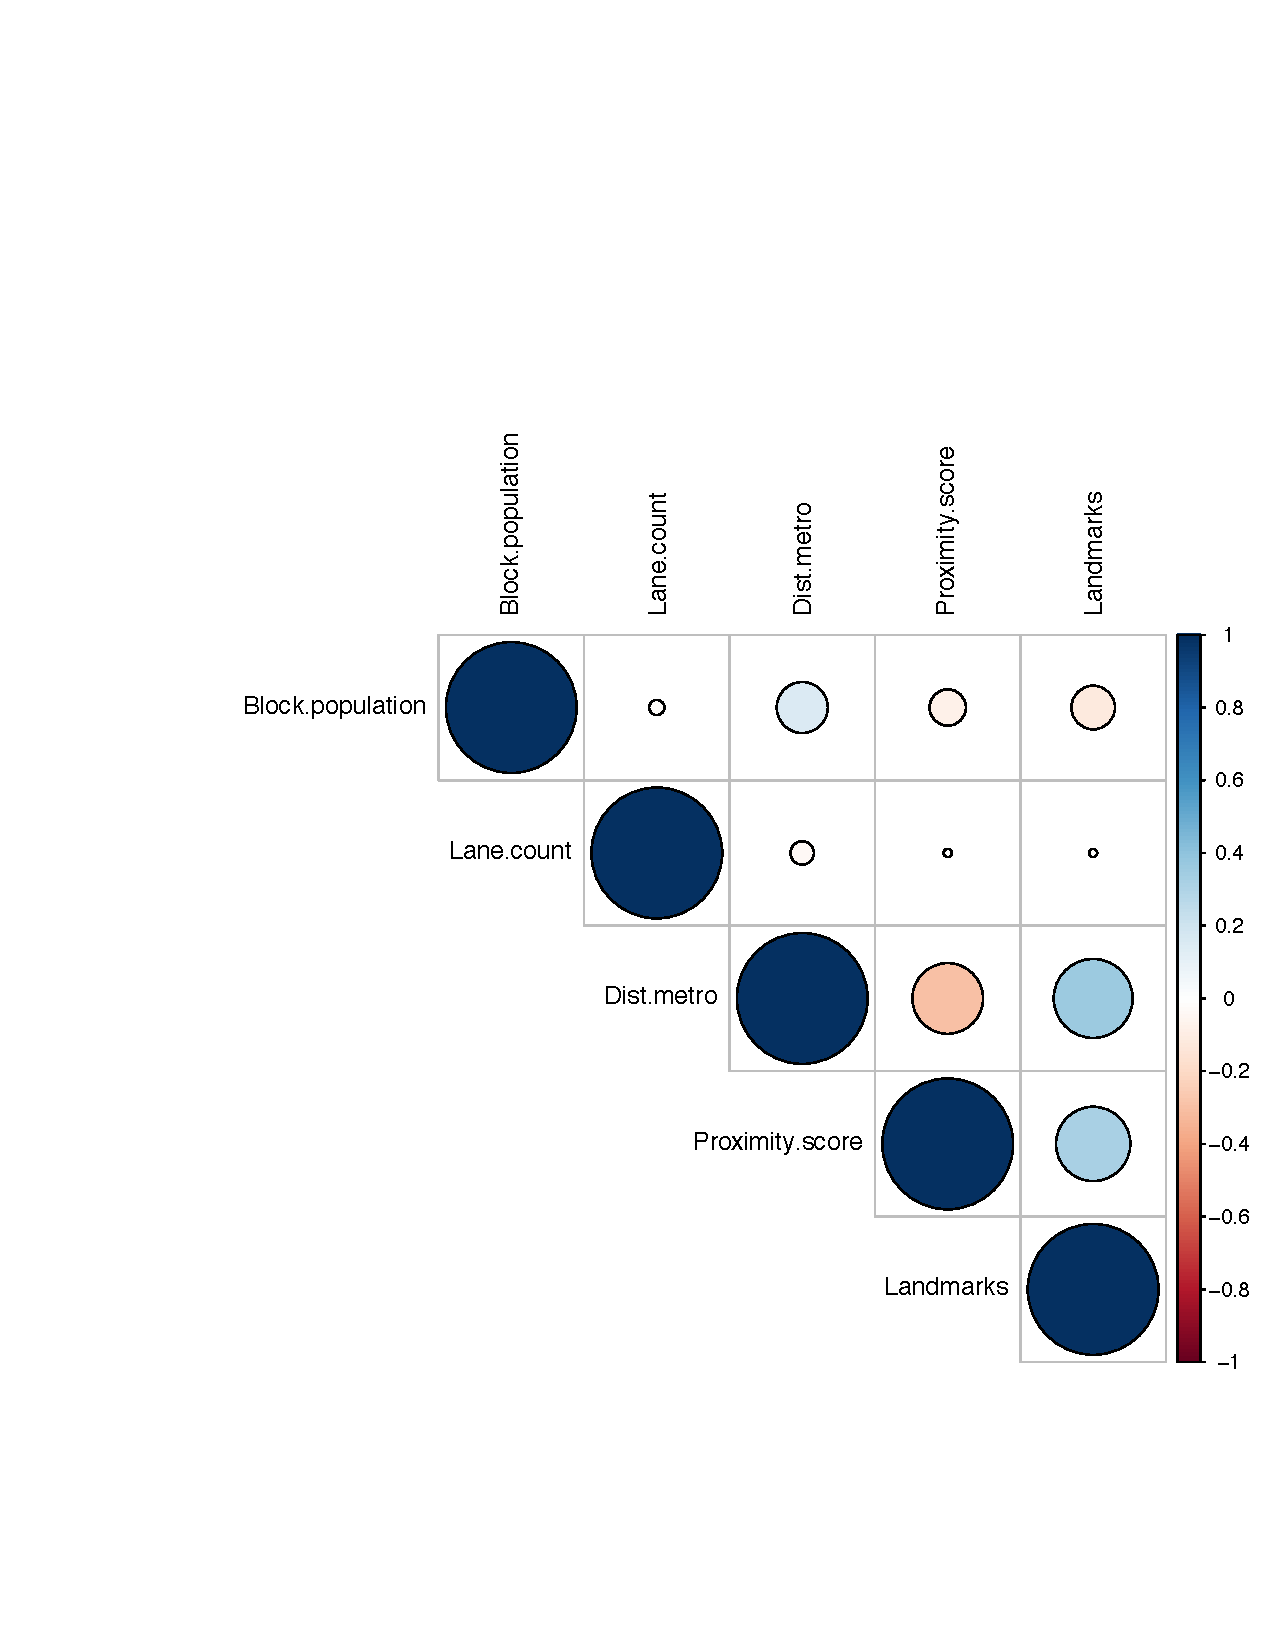
\includegraphics[scale=0.7]{Pictures/corrplot}
	\caption{Correlation matrix between predictors}\label{corrplot}
\end{figure}


\subsection{Setup of the model variants}

We evaluated the performance of previously described point-referenced Gaussian model by varying the (sub)set of predictors included, according to the following table.
\begin{table}[H]
	\centering
	\begin{tabular*}{0.75\textwidth}{ r|c|c|c|c|c| }
	\multicolumn{1}{r}{}
	&  \multicolumn{1}{c}{Population}
	&  \multicolumn{1}{c}{Lanes} 
	&  \multicolumn{1}{c}{Subway}
	&  \multicolumn{1}{c}{Proximity}
	&  \multicolumn{1}{c}{Landmarks} \\
	\cline{2-6}
	Model 1 & $\checkmark$ & $\checkmark$ & $\checkmark$ &  & \\
	\cline{2-6}
	Model 2 & $\checkmark$ & $\checkmark$ & $\checkmark$ & $\checkmark$ & \\
	\cline{2-6}
	Model 3 & $\checkmark$ & $\checkmark$ & $\checkmark$ & $\checkmark$ & $\checkmark$ \\
	\cline{2-6}
	Model 4 & $\checkmark$ & $\checkmark$ & $\checkmark$ &  & $\checkmark$ \\
	\cline{2-6}
	\end{tabular*}
	\caption{Models setup}
\end{table}

\noindent
A further division for evaluating different models has been performed over space, concerning the definition of the training sets, and consequently of the testing sets on which model validation was performed via prediction. This is further discussed later. The two different training and testing sets are shown in Figure \ref{southset} and Figure \ref{bothset}. With this choice, it is possible to check how the model performs:
	\begin{enumerate}[label=(\arabic*)]
		\item  When it is trained using data from Southern Manhattan peninsula, where a major part of sites of interest is located, and 
		\item  When it is trained by using data from the Southern and the Northern part of town, given that the latter is mainly residential compared to the others, plus demand is fairly lower.
	\end{enumerate}
	Using both training sets enclosed in red boxes, the next step is to test the model on the Central part of Manhattan, which is approximately the area inside the green box.
	The motivation for choosing these divisions follows the preliminary observed distribution of the demand. Indeed, it is almost symmetric with respect to the center, but quite ``heavier" towards the Southern edge.
	\vspace{3 mm}
	\begin{figure}[H]
		\centering
		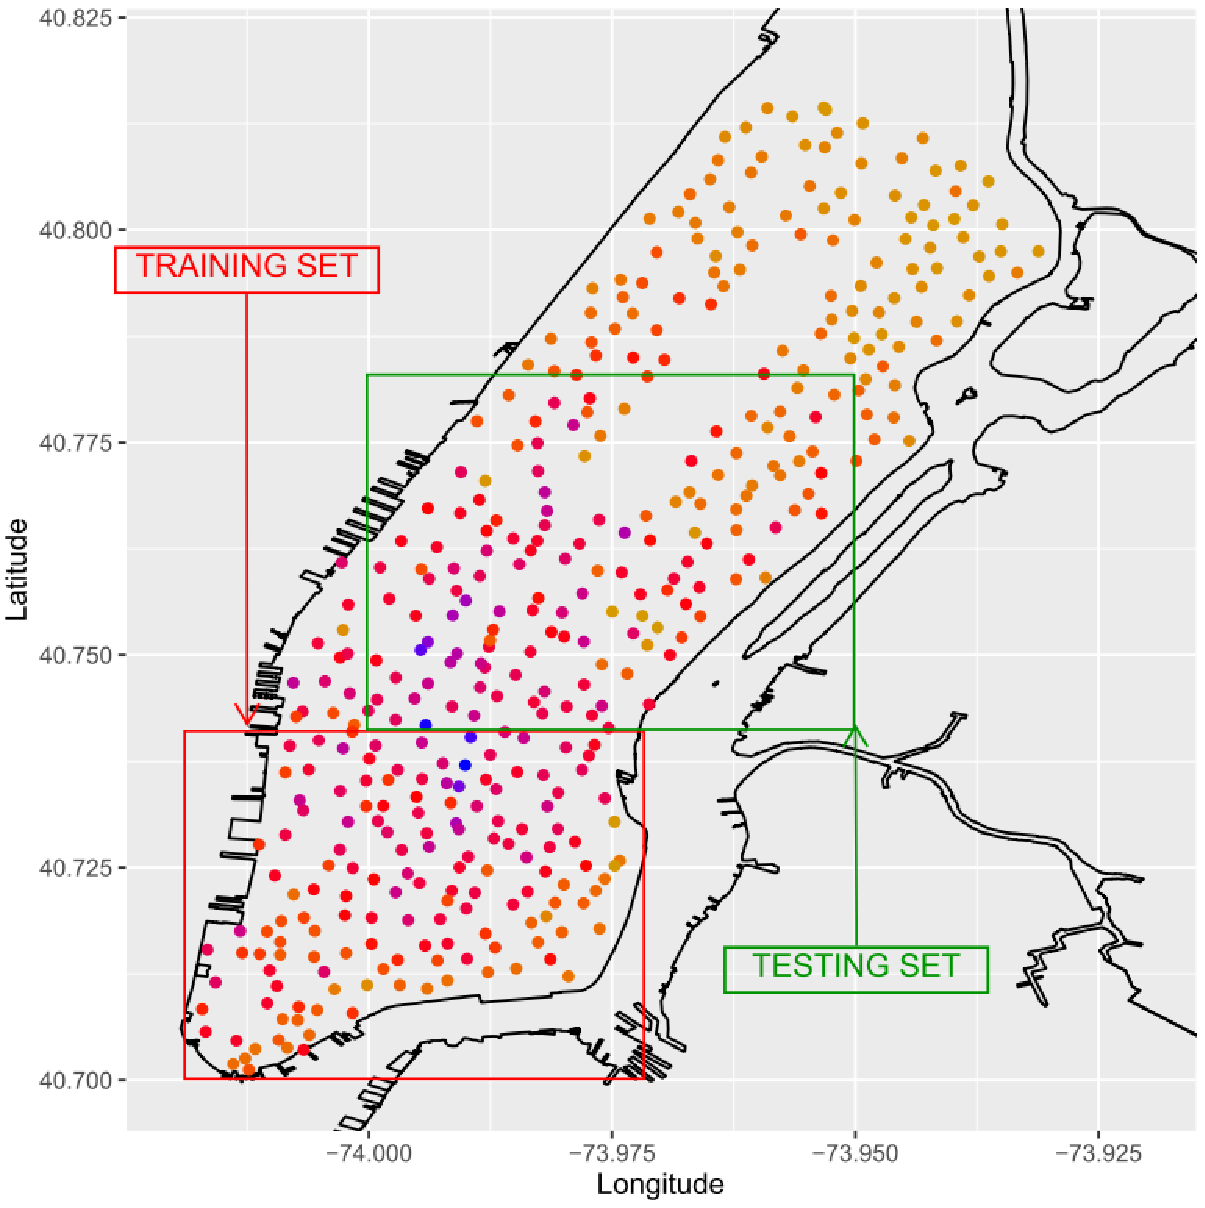
\includegraphics[scale=0.5]{Pictures/manhattan_map_test1.pdf}
		\caption{First (South) training set}\label{southset}
	\end{figure}
	\vspace{3 mm}
	\begin{figure}[H]
		\centering
		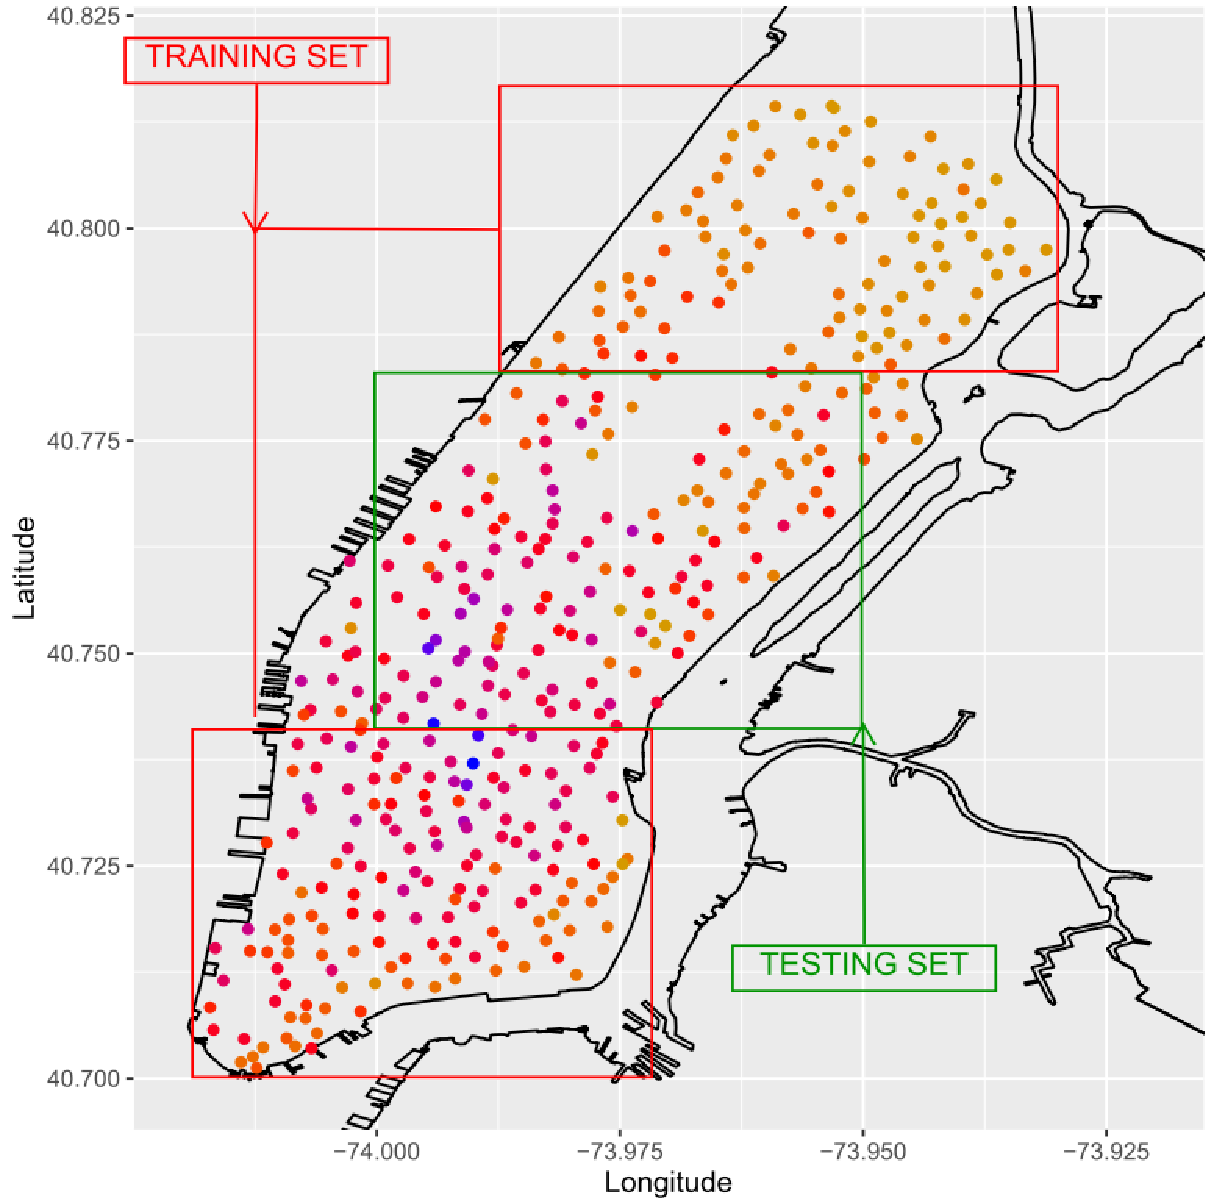
\includegraphics[scale=0.5]{Pictures/manhattan_map_test2.pdf}
		\caption{Second (South+North) training set}\label{bothset}
	\end{figure}



\subsection{Comparing the different models}
\subsubsection{Predictive goodness of fit}
For the location $\{\mathbf{s}_i : i=1,\dots,n\}$, we computed the following goodness of fit criteria for all the models presented previously:
\begin{itemize}
\item Log Pseudo Marginal Likelihood (LPML):
$$LPML = \sum_{i=1}^n \log{CPO(\mathbf{s}_i)}$$
where the Conditional Predictive Ordinate (CPO) are approximated with posterior samples $\{\boldsymbol{\theta}^{(k)} \}_{k=1}^K$ as follows
$$(CPO(\mathbf{s}_i))^{-1} \approx \frac{1}{K} \sum_{k=1}^K \frac{1}{f(y(\mathbf{s}_i) | \boldsymbol{\theta}^{(k)})}$$
with $f(\cdot \,|\, \boldsymbol{\theta}^{(k)})$ posterior density defined by means of draws $\boldsymbol{\theta}^{(k)}$.
\item Watanabe-Akaike Information Criterion (WAIC):
$$WAIC = -2(lppd_{computed}-p_{WAIC})$$
where the $p_{WAIC}$ refers to the sample variance from a MCMC of the log pointwise predictive density, and $lppd_{computed}$ is computed via MCMC with M draws as follows 
 $$lppd_{computed}= \sum_{1}^nlog( \frac{1}{M}\sum_{j=1}^{M}f_{i}(y(\mathbf{s}_i) | \boldsymbol{\theta}^{(j)})$$
\end{itemize}


The results are shown in Table \ref{gof_results}.


\renewcommand{\baselinestretch}{1.5}
\begin{table}[H]
\centering
\begin{tabular}{cccccc}
%\cline{3-6}
&& Model 1 & Model 2 & Model 3 & Model 4 \\ \cline{2-6}
\multicolumn{1}{c|}{\multirow{2}{*}{South}} & \multicolumn{1}{c|}{LPML} & -2140.44 & -2140.45 & -2139.74 & \multicolumn{1}{c|}{\textbf{-2133.71}} \\
\multicolumn{1}{c|}{} & \multicolumn{1}{c|}{WAIC} & 4280.85 & 4280.87 & 4279.47 & \multicolumn{1}{c|}{\textbf{4267.28}} \\
\cline{2-6}
\multicolumn{1}{c|}{\multirow{2}{*}{South+North}} & \multicolumn{1}{c|}{LPML} & -3579.91 & -3576.97 & \textbf{-3574.97} & \multicolumn{1}{c|}{-3575.53} \\
\multicolumn{1}{c|}{} & \multicolumn{1}{c|}{WAIC} & 7159.82 & 7153.93 & \textbf{7149.94} & \multicolumn{1}{c|}{7151.06} \\
\cline{2-6}
\end{tabular}
\caption{Goodness of fit criteria}\label{gof_results}
\end{table}
 \renewcommand{\baselinestretch}{1}

\noindent
For each training set, models having the maximum LPML and minimum WAIC are marked.

\section{Results}
\subsection{Models performance}

\noindent
We have computed the posterior densities of our models obtained from the two training regions. We here deduce some preliminary conclusions, analyzing first coefficients, then discussing covariance parameters.\\

\subsubsection{Posterior coefficient parameters}
	In general, we see that different traceplots for the model coefficients $\boldsymbol{\beta}$ vary over all the range uniformly indicating the well-posedness of the problem. Moreover, by checking the densities obtained we could state that they well approximate Gaussian distributions.\\
	
	\noindent
	On one hand, the positive value of the intercept suggests that the creation of a new station will be advisable generating a positive demand.  Additionally, places near important landmarks would take advantage of this fact.\\
	
	\noindent
	On the other hand, we should take into account the fact that the proximity between stations decreases their demands. Furthermore, the existence of other facilities such as subways on the surroundings reduces the use of bikes as well.\\
	
	\noindent
	As a demonstrative example, we report in Figure 7 posterior densities and for model coefficients $\boldsymbol{\beta}$ from Model 3 (using all the defined covariates). Their behavior for all models looks like this.

\begin{figure}[H]
		\centering
		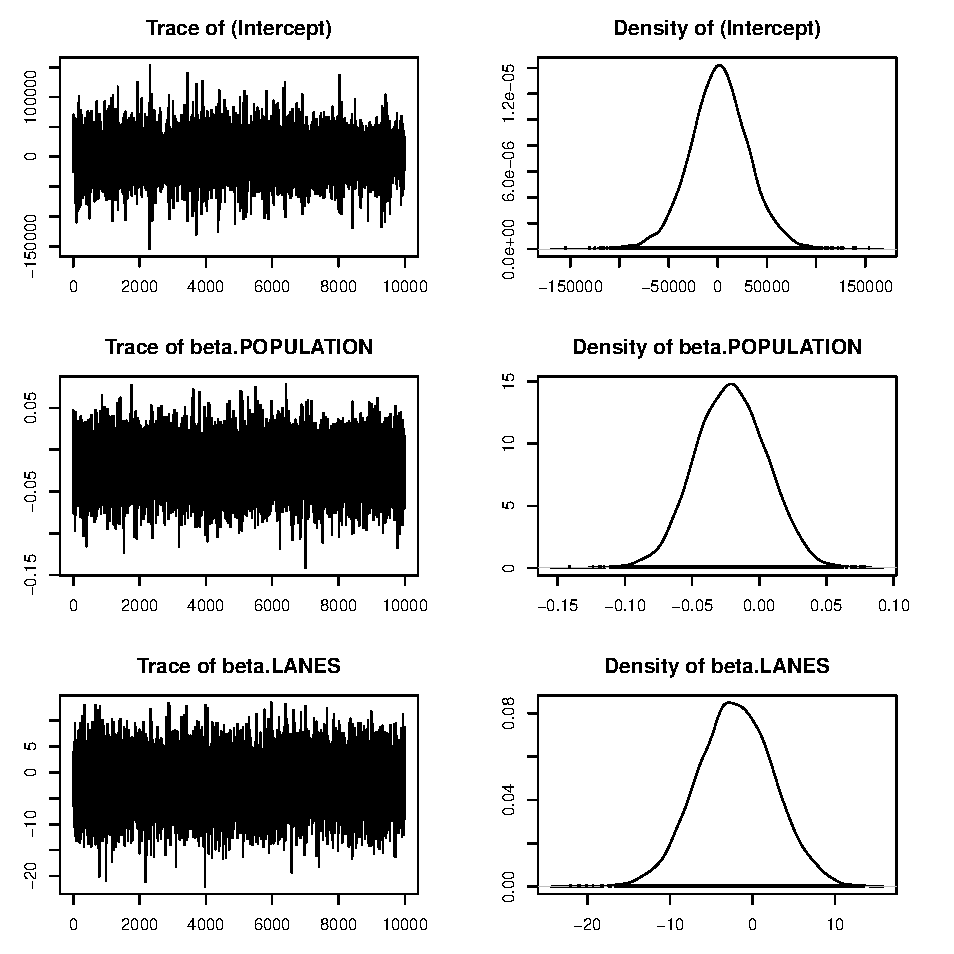
\includegraphics[scale=0.55]{Pictures/beta_1.pdf}
		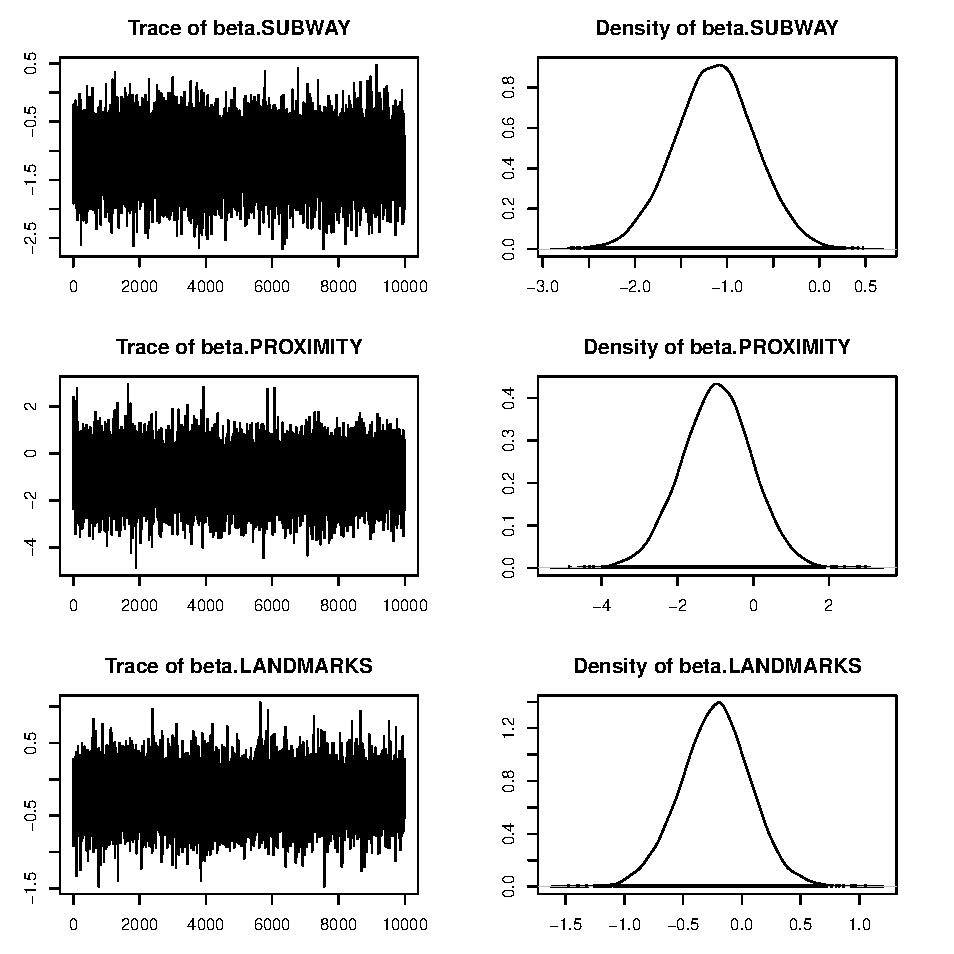
\includegraphics[scale=0.55]{Pictures/beta_2.pdf}
		\caption{Traceplots and densities of the posterior coefficients}
\end{figure}


\subsection{Posterior covariance parameters and chain diagnostics}
	Function \emph{spLM} employed to create these models works by sampling via a random walk Metropolis Hastings algorithm, and it requires for each run a set of tuning parameters ${\sigma^2}_{tun}$, ${\tau^2}_{tun}$ and ${\phi}_{tun}$ for each of the three covariance parameters. The initial choice of these is strongly responsible for how well the Markov Chain constructed converges, besides being fundamental for establishing its acceptance rate. \\
	
	\noindent
	In our case, the choice made following several attempts was: \\
	\begin{itemize}
		\item For models on traning set (South): ${\sigma^2}_{tun} = 0.15$, ${\tau^2}_{tun} = 0.2$, ${\phi}_{tun} = 3$
		\item For models on training set (South+North): ${\sigma^2}_{tun} = 0.05$, ${\tau^2}_{tun} = 0.05$, ${\phi}_{tun} = 5$
	\end{itemize}
	\vspace{3 mm}
	Such choices allowed the acceptance rate of the algorithm to be on average between 22 and 25\% for all models (more details in Table \ref{accept}). Trace and autocorrelation function plots shown in the next pages are relative to the second experiment on training set (South+North), and have been obtained from simulating $n=20000$ samples.\footnotemark
	
	\footnotetext{More plots on cumulative mean and summaries of posterior distribution can be retrieved from the code}
	\begin{figure}[H]
		\centering
		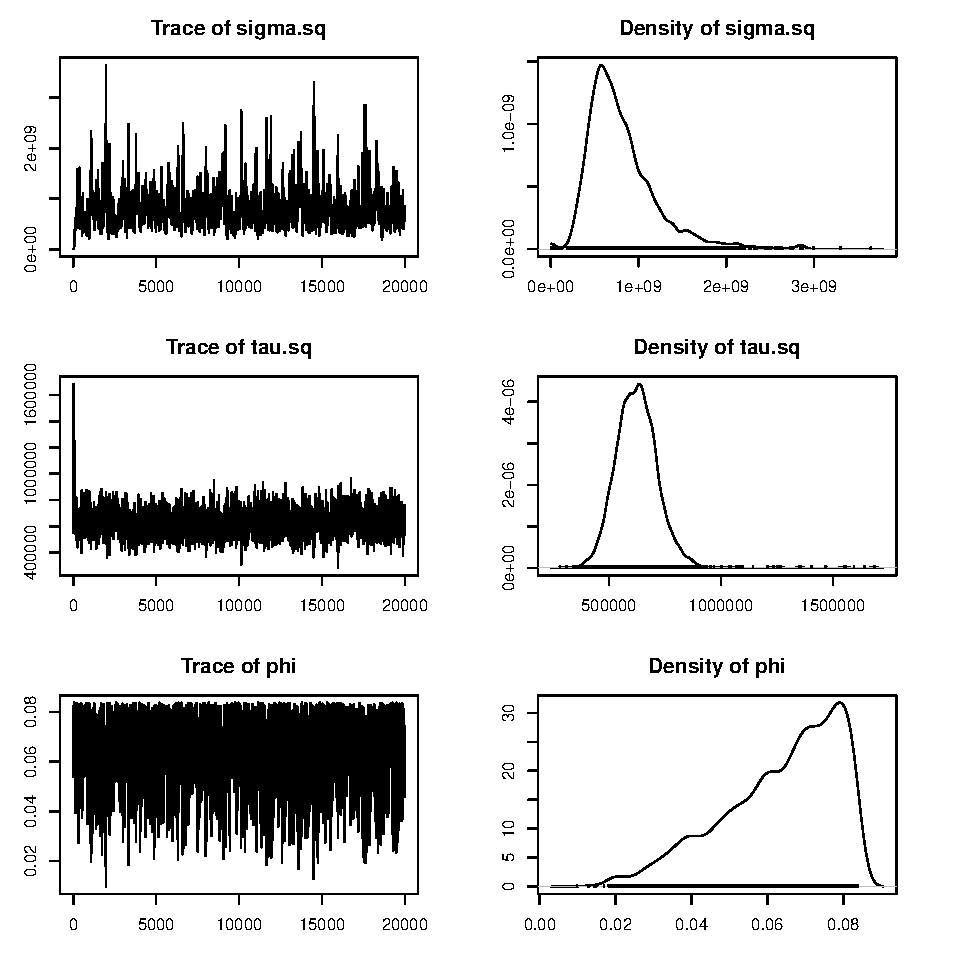
\includegraphics[scale=0.55]{Plots_North+South/v1_both.pdf}
		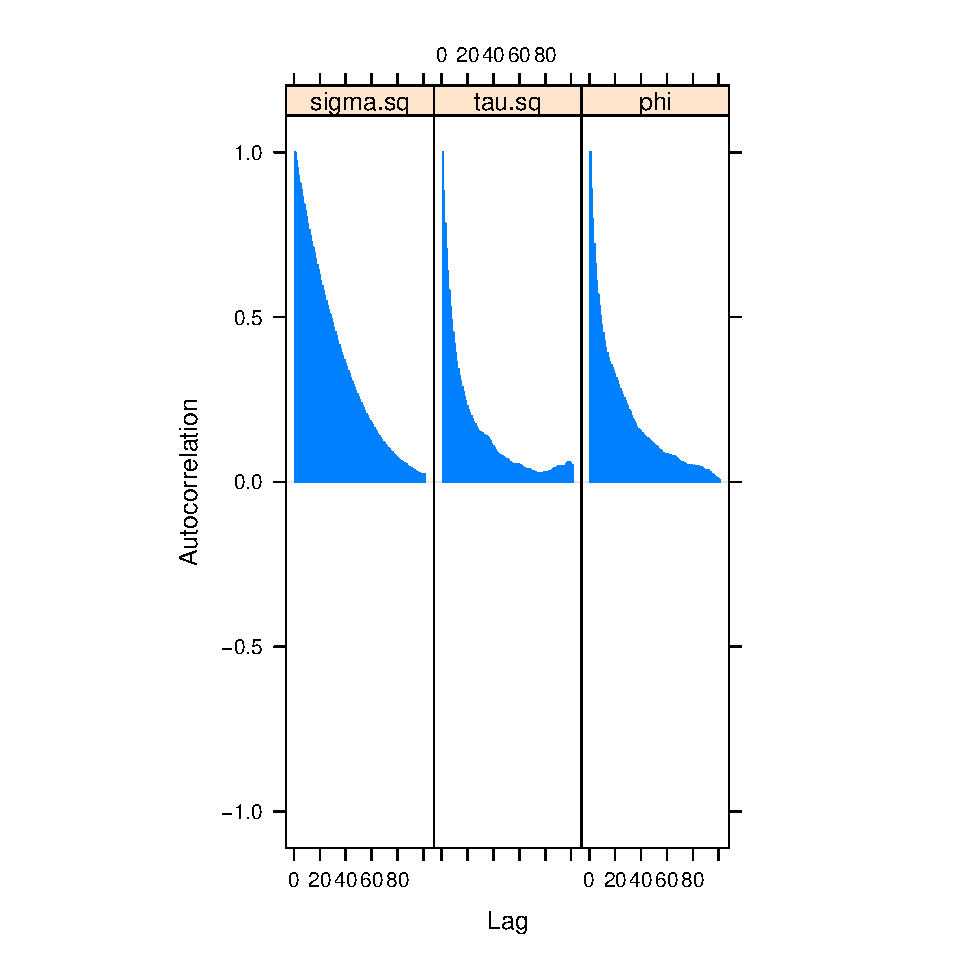
\includegraphics[scale=0.55]{Plots_North+South/v1_both_acf.pdf}
		\caption{Trace plots, posteriors and ACF plots for Model 1}
	\end{figure}
	
	\begin{figure}[H]
		\centering
		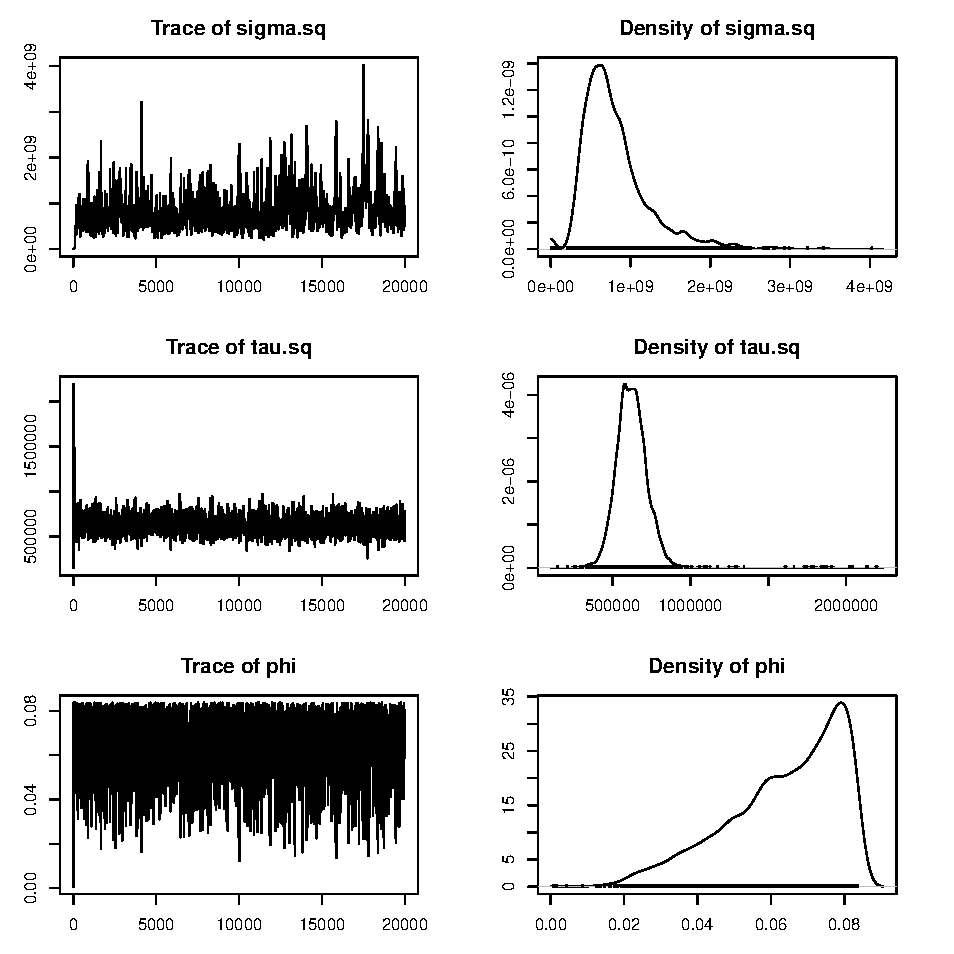
\includegraphics[scale=0.55]{Plots_North+South/v2_both.pdf}
		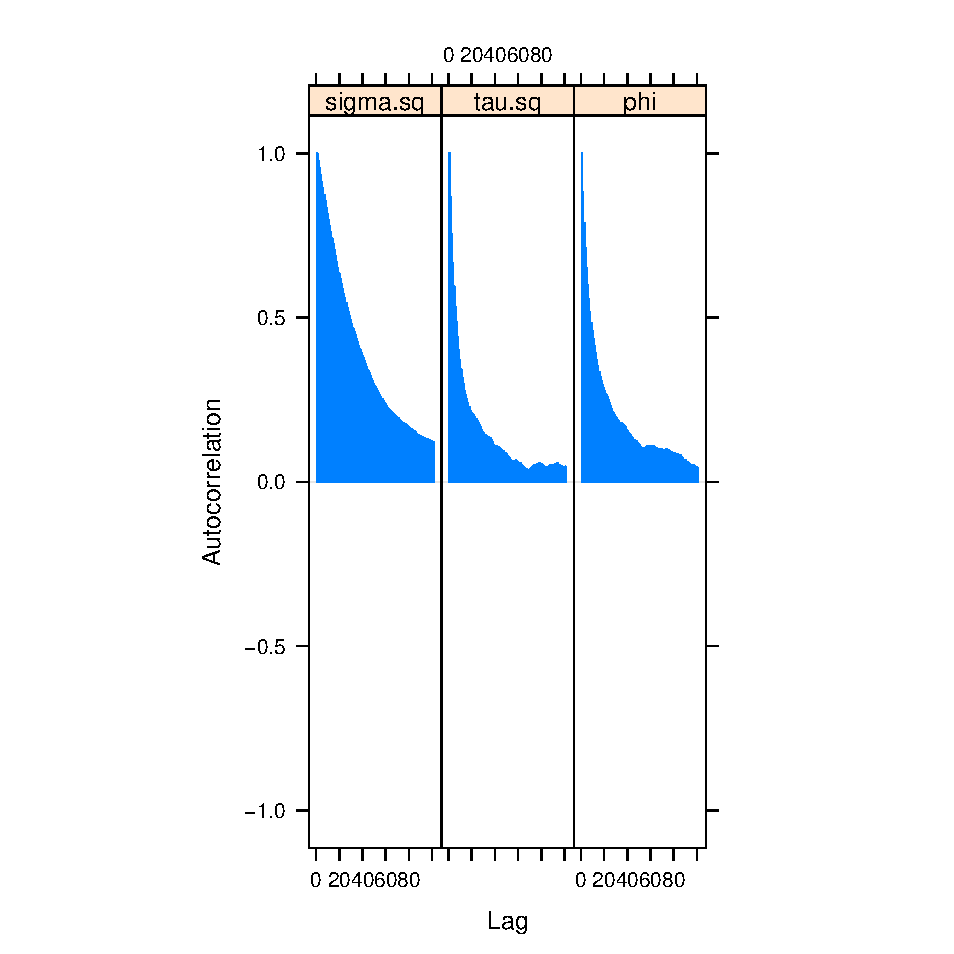
\includegraphics[scale=0.55]{Plots_North+South/v2_both_acf.pdf}
		\caption{Trace plots, posterior densities and ACF plots for Model 2}
	\end{figure}
	
	\begin{figure}[H]
		\centering
		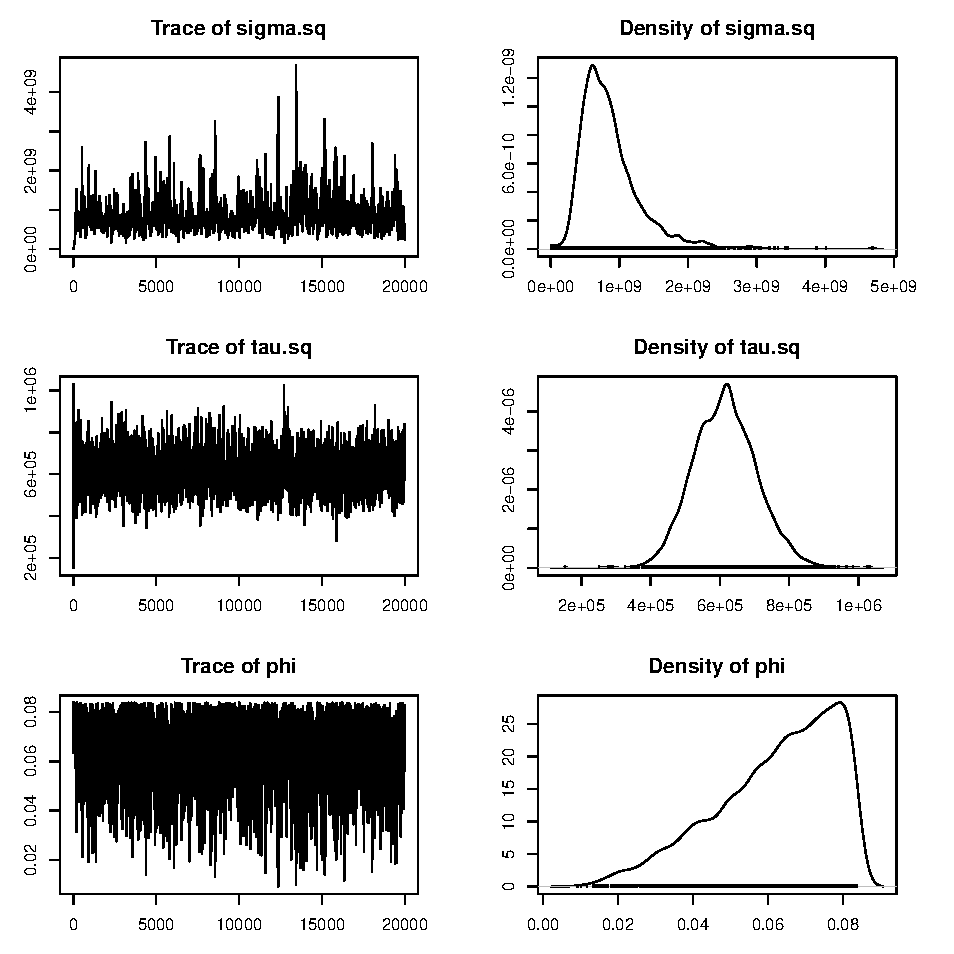
\includegraphics[scale=0.55]{Plots_North+South/v3_both.pdf}
		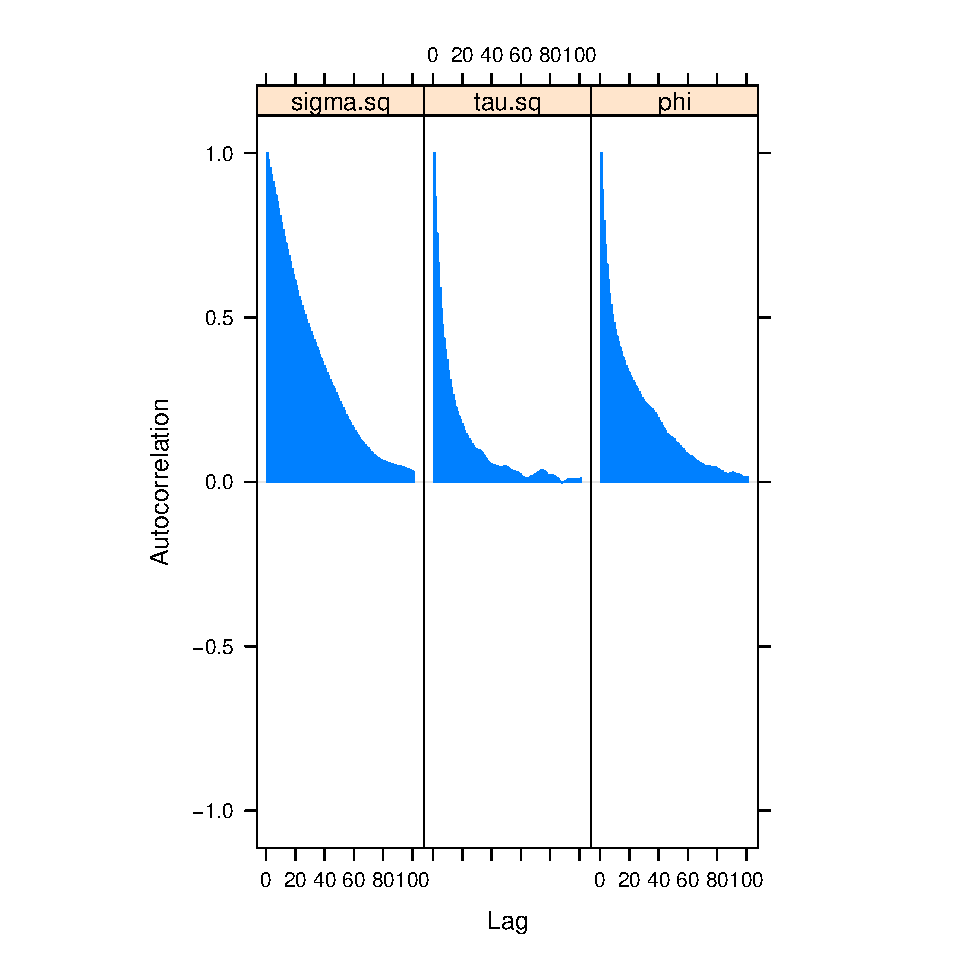
\includegraphics[scale=0.55]{Plots_North+South/v3_both_acf.pdf}
		\caption{Trace plots, posterior densities and ACF plots for Model 3}
	\end{figure}
	
	\begin{figure}[H]
		\centering
		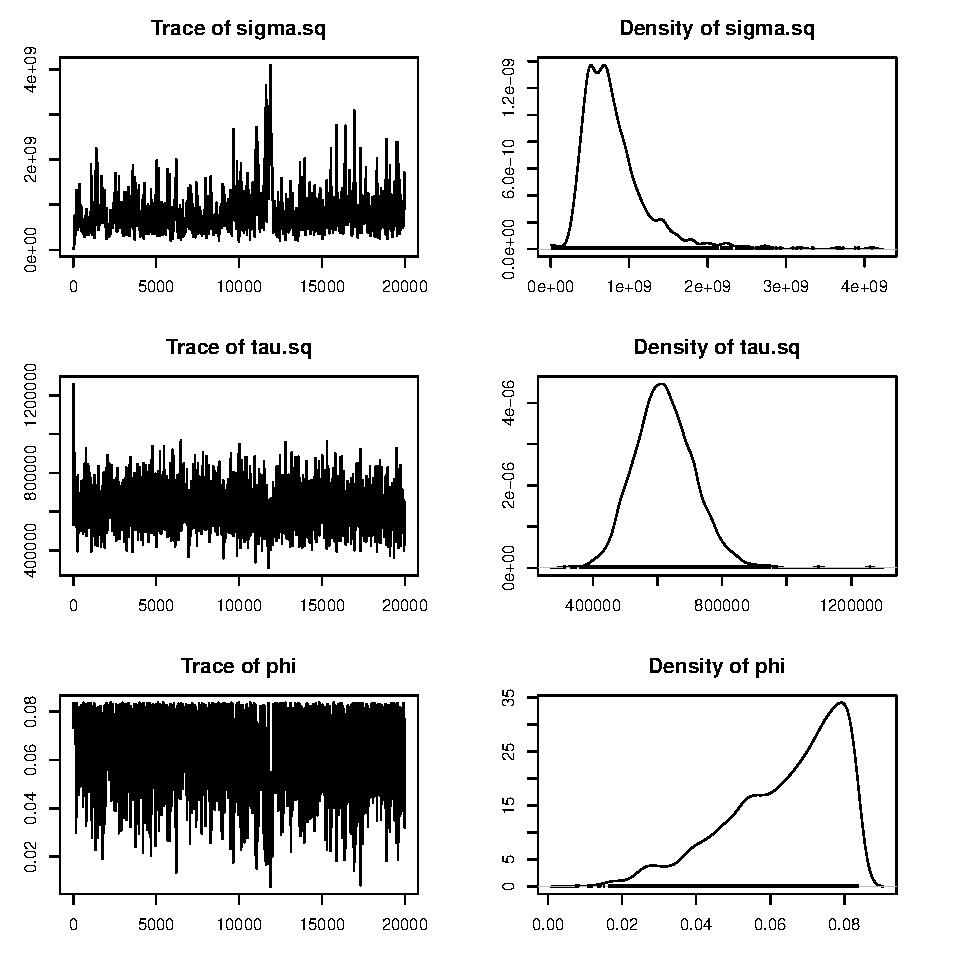
\includegraphics[scale=0.55]{Plots_North+South/v4_both.pdf}
		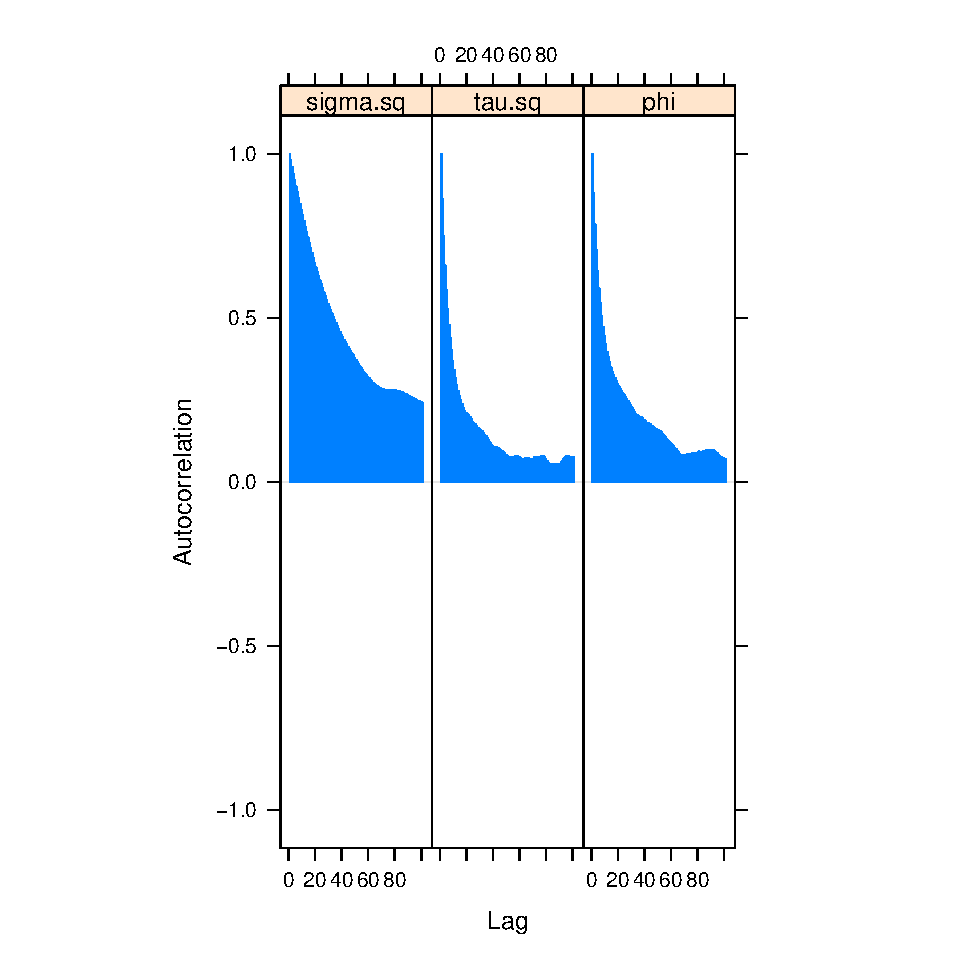
\includegraphics[scale=0.55]{Plots_North+South/v4_both_acf.pdf}
		\caption{Trace plots, posterior densities and ACF plots for Model 4}
	\end{figure}

	\noindent
	Due to the preliminary choice of considering residual variances from a linear model fit in the priors for $\sigma^2$ and $\tau^2$, their posteriors appear to be spread widely, meaning that a very low value of density corresponds to each point.\\
	
	\noindent
	So far, the chain produces better results when using training set (South+North), probably thanks to the larger number of observations and thus to a wider exploration of the domain that partly help spatial process parameters'
	autocorrelation lag to reduce faster through the sampling process. The traces seem to have a few high peaks especially for $\sigma^2$, but still exploring fairly the state space.\\
	
	\noindent
	From Table \ref{effsize}, an estimate for the number of independent samples generated by the chain is provided, as returned by R function \emph{effectiveSize}.
	\renewcommand{\baselinestretch}{1.5}
	\begin{table}[H]
		\centering
		\begin{tabular}{cccccc}
			%\cline{3-6}
			&& Model 1 & Model 2 & Model 3 & Model 4 \\ \cline{2-6}
			\multicolumn{1}{c|}{\multirow{3}{*}{South}} & \multicolumn{1}{c|}{ $\sigma^2$} & 312.99 & 345.88 & 296.55 & \multicolumn{1}{c|}{197.13} \\
			\multicolumn{1}{c|}{} & \multicolumn{1}{c|}{$\tau^2$} & 849.08 & 495.07 & 106.03 & \multicolumn{1}{c|}{107.33} \\
			\multicolumn{1}{c|}{} & \multicolumn{1}{c|}{$\phi$} & 800.10 & 955.42 & 744.80 & \multicolumn{1}{c|}{537.61}\\
			\cline{2-6}
			\multicolumn{1}{c|}{\multirow{3}{*}{South+North}} & \multicolumn{1}{c|}{$\sigma^2$} & 247.21 & 235.19 & 272.78 & \multicolumn{1}{c|}{208.05} \\
			\multicolumn{1}{c|}{} & \multicolumn{1}{c|}{$\tau^2$} & 848.74 & 796.96 & 1061.22 & \multicolumn{1}{c|}{811.28} \\
			\multicolumn{1}{c|}{} & \multicolumn{1}{c|}{$\phi$} & 562.56 & 640.26 & 517.19 & \multicolumn{1}{c|}{557.84} \\
			\cline{2-6}
		\end{tabular}
		\caption{Effective sample size compared}\label{effsize}
	\end{table}
	\renewcommand{\baselinestretch}{1}
	
	\noindent
	Overall the larger training set seems to perform better. The main differences on sample size between (South) and (South+North) can be observed for $\tau^2$ in Model 3 and Model 4, very likely because of the particular choice of the tuning parameters.\\

	\noindent
	The global acceptance rate achieved is not quite high, as shown in Table \ref{accept}. However with our choice of tuning parameters and priors, there was some trade-off between acceptance, performance of trace plots and convergence. By choosing larger tuning parameters for the process variances $\sigma^2$ and $\tau^2$, the algorithm would have a higher acceptance rate, but the efficiency would not be significantly improved.
	
	\renewcommand{\baselinestretch}{1.5}
	\begin{table}[H]
		\centering
		\begin{tabular}{ccccc}
			& Model 1 & Model 2 & Model 3 & Model 4 \\ 
			\cline{2-5}
			\multicolumn{1}{c|}{Model 1} & 22.62 & 22.80 & 23.40 & \multicolumn{1}{c|}{23.67} \\
			\cline{2-5}
			\multicolumn{1}{c|}{Model 2} & 24.86 & 25.19 & 25.02 & \multicolumn{1}{c|}{25.79} \\
			\cline{2-5}
		\end{tabular}
		\caption{Global Metropolis acceptance rate compared(\%)}\label{accept}
	\end{table}
	\renewcommand{\baselinestretch}{1}

\subsection{Prediction}

Once determined the posterior distributions, we made some predictions using function \emph{spPredict}.\\

\noindent
As previously introduced, we followed two approaches in order to train our model. We considered a unique training set (South) and a joint training set (South+North) with the aim of taking into account the diverse evolution of the demand.
In both cases, we used the center of Manhattan as test set, having the observed demand in Figure \ref{observed}.\\
\vspace{3 mm}
\begin{figure}[H]
		\centering
		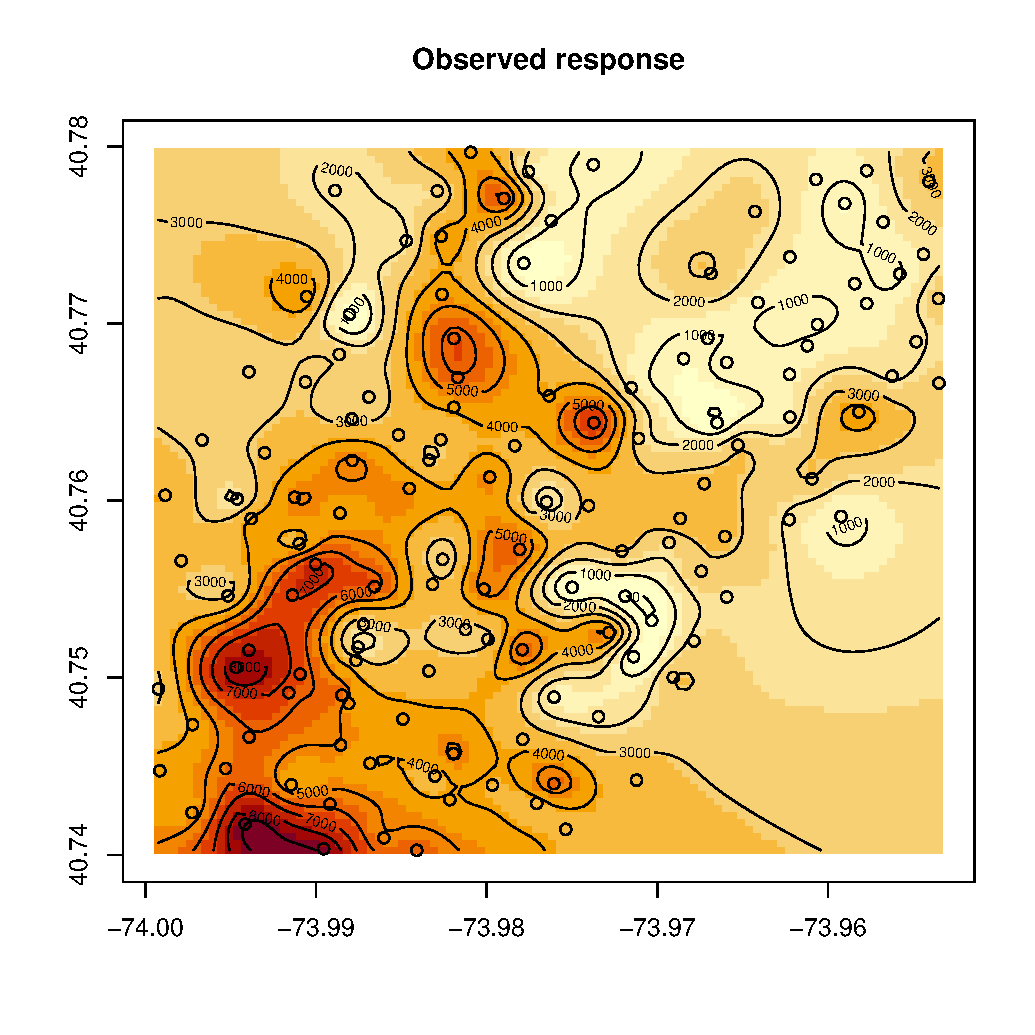
\includegraphics[scale=0.50]{Pictures/Obs_centre_map.pdf}
		\caption{Observed demand in central Manhattan}\label{observed}
\end{figure}

\noindent
Initiatlly, in order to select the best one of the two approaches, we have predicted the demand behavior on the test set by applying our model on a fixed grid of points. This has been done specifically for Model 1 and Model 4, since they do not contain the Proximity covariate. In figure \ref{pred1} are shown results from Model 1 \\

\begin{figure}[H]
		\centering
		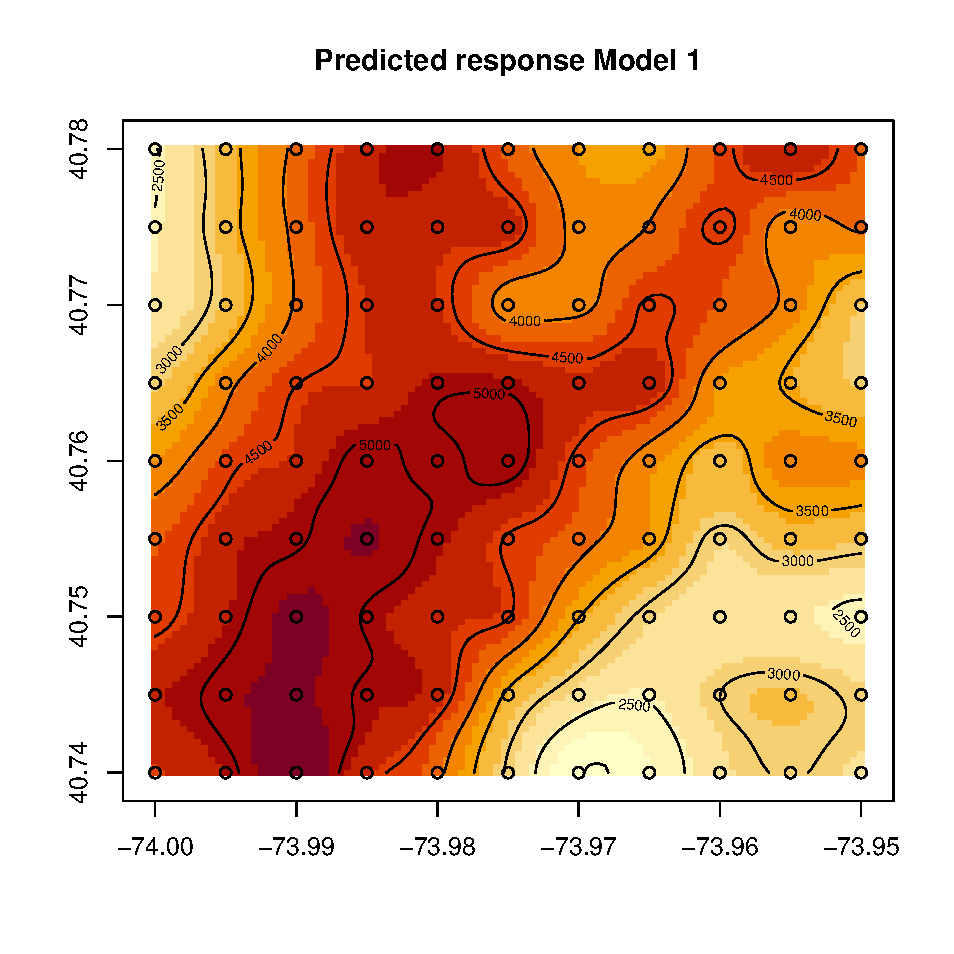
\includegraphics[scale=0.50]{Plots_South/v1_south_pred_grid.pdf}
		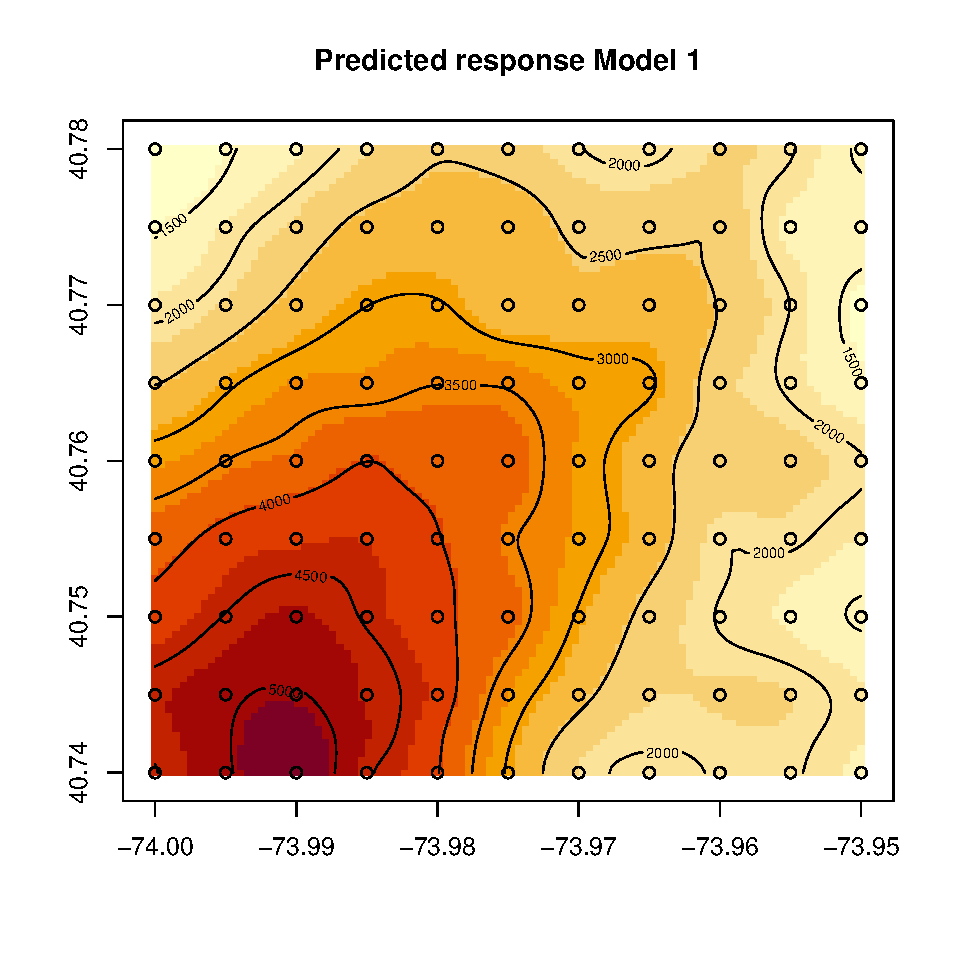
\includegraphics[scale=0.50]{Plots_North+South/v1_both_pred_grid.pdf}
		\caption{Prediction on training set (South) on the left, (South+North) on the right}\label{pred1}
\end{figure}

\noindent
When comparing grid predictions, we see that the gradient is more regular when using the larger training set (South+North), distinguishing better those zones with less demand, whereas from the (South) training set a higher mean demand all over the map was forecasted.\\

\noindent
Finally, we also performed the prediction on the points where actual stations are. To give an idea of how the prediction looks like when performed on real points versus on a grid of points, we show this comparison again for Model 1 performance in Figure \ref{pred2}. On the contrary of the previous, this procedure has been applied for all the four models, careless of their predictors. \\


\begin{figure}[H]
	\centering
	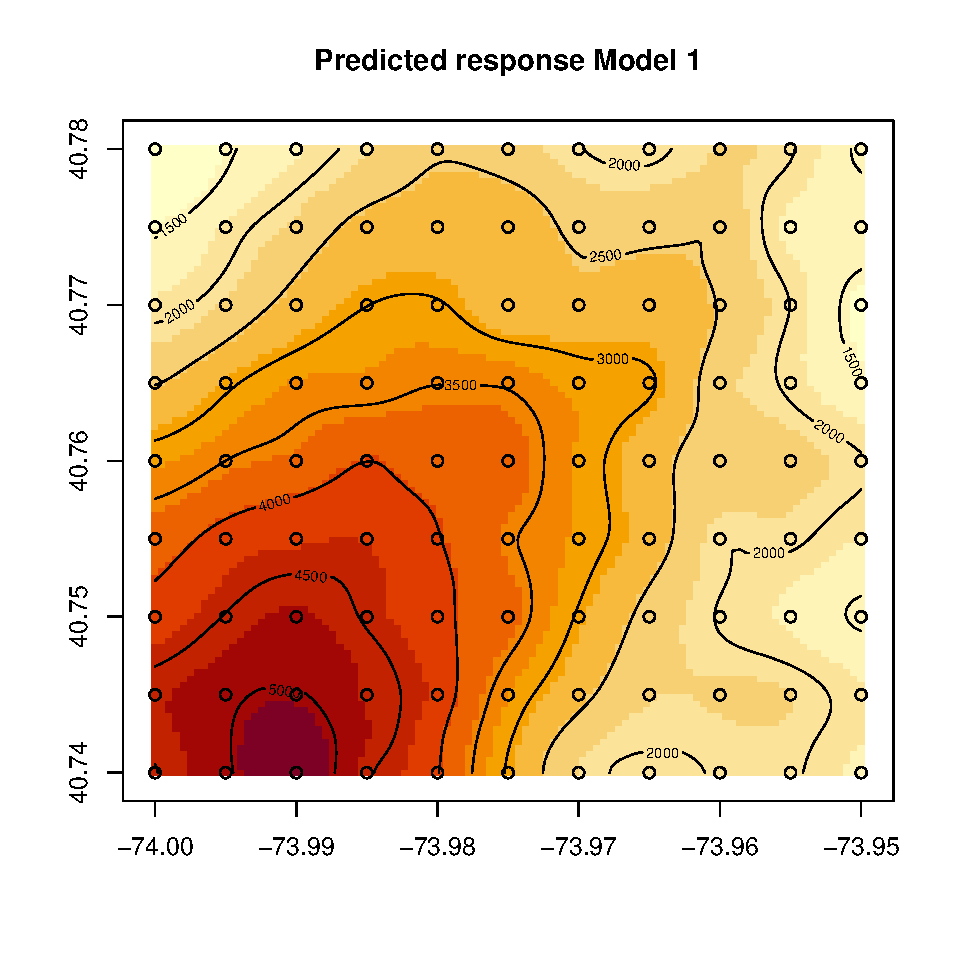
\includegraphics[scale=0.50]{Plots_North+South/v1_both_pred_grid.pdf}
	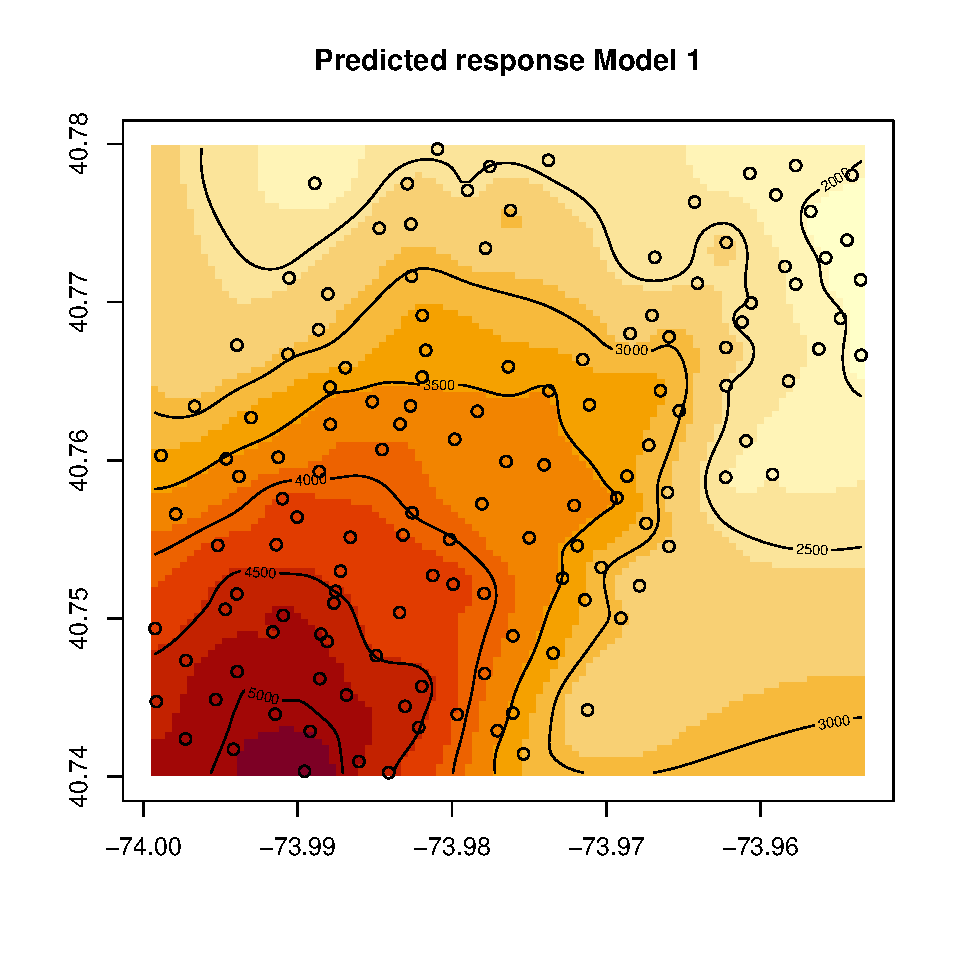
\includegraphics[scale=0.50]{Plots_North+South/v1_both_pred_stations.pdf}
	\caption{Prediction on grid on the left, at exact stations on the right}\label{pred2}
\end{figure}

\noindent
With this differentiation all the different models behave quite similar. We could state that the best prediction balance appears to be that of Model 3. The darker color representing higher demand dominates the Southern edge of the picture, while towards the North the predicted demand gradually decreases, very likely to the real observed data at station points.\\
\begin{figure}[H]
		\centering
		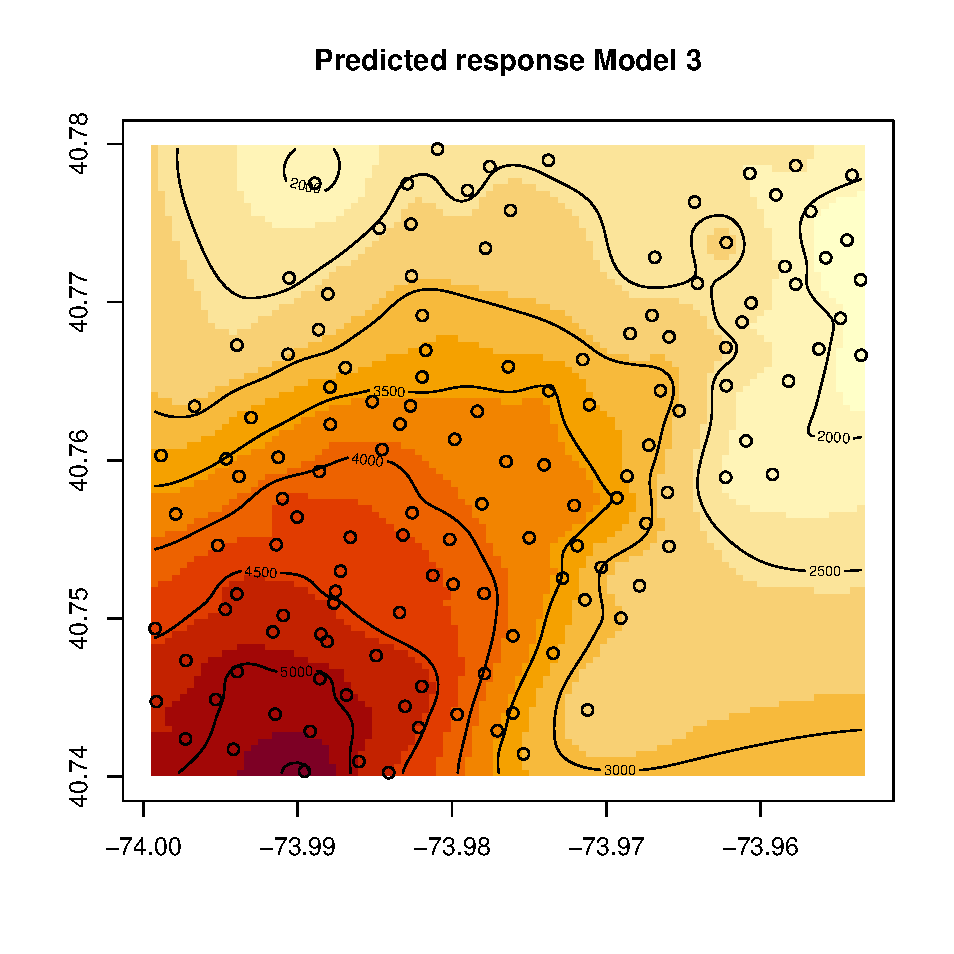
\includegraphics[scale=0.5]{Plots_North+South/v3_both_pred_stations.pdf}
		\caption{Predicted demand at stations in central Manhattan from Model 3}
\end{figure}
\noindent
Overall, the forecast provided using all the models is smooth. 
\footnote{The complete set of plots can be found is in the folders "South" and "North+South" in the Github repository}\\

\noindent
As a general conclusion it can be acknowledged that observed pattern distinguish properly places, and ultimately stations, with higher demand from those with less, in a quite realistic way, according to the data available on Manhattan stations. The predictive performance of all the models experimented is satisfactory.
 
 








\begin{flushleft}
	\begin{thebibliography}{9}
	\bibitem{manhattan}
	Moss M.L., Qing C.,
	\textit{The Dynamic Population of Manhattan},
	Rudin Center for Transportation Policy and Management,	
	Wagner School of Public Service,
	New York University,
	(2012).
	\bibitem{hierarchical}
	Banjeree S., Carlin B.P., Gelfand A.E.,
	\textit{Hierarchical modeling and analysis for spatial data},
	Second edition,
	(2014).
	\bibitem{spbayes}	
	Finley A.O., Banjeree S., Gelfand A.E.,
	\textit{spBayes for Large Univariate and Multivariate Point-Referenced Spatio-Temporal Data Models},
	Journal of Statistical Software,
	Volume 63, Issue 13,
	(2015).
	\bibitem{bayesgaussian}
	Shuvo Bakar K., Kokic P.,
	\textit{Bayesian Gaussian Models for Point-Referenced Spatial and Spatio-Temporal data}
	Journal of Statistical Research,
	Volume 51, No.1, pp.17-40,
	(2017).
	\bibitem{isotropytest}
	Weller Z.D.,
	\textit{spTest: an R Package imlementing Nonparametric Tests of Isotropy},
	(2018).
	\bibitem{carbayes}
	Lee D.,
	\textit{CARBayes version 5.1.3: An R Package for Spatial Areal Unit Modelling with Conditional Autoregressive Priors},
	University of Glasgow,
	(2013).
	\bibitem{maity}
	Maity A., Sherman M.
	\textit{Testing for spatial isotropy under general designs. Journal of Statistical Planning and Inference}, 
	142(5), 1081-1091,
	(2012).
	\bibitem{stationdata}
	Citi Bike System Data : \emph{https://www.citibikenyc.com/system-data}
	\bibitem{lanesdata}
	Bicycle Routes | NYC Open Data: \emph{https://data.cityofnewyork.us/Transportation/Bicycle-Routes/7vsa-caz7}
	\bibitem{subwaydata}
	Subway Stations | NYC Open Data:
	\emph{https://data.cityofnewyork.us/Transportation/Subway-Stations/arq3-7z49},
	CSV file
	\bibitem{populationdata}
	2010 Census Tracts | NYC Open Data:
	\emph{https://data.cityofnewyork.us/City-Government/2010-Census-Tracts/fxpq-c8ku},
	CSV file
	
	
\end{thebibliography}

\end{flushleft}
\end{document}